%\documentclass[12pt]{scrreprt}
\documentclass[12pt]{report} 

% language may be romanian or english (default is english)
% type may be bachelor or master (default is bachelor)
\usepackage[language=romanian, type=bachelor]{style}

\usepackage{subcaption} %so we can do subfigures

\usepackage{float} %so that we have the H option available

%\geometry{a4paper,top=2.5cm,left=3cm,right=2.5cm,bottom=2.5cm}
%in style
%controlling the appearance of your headers and footers
\usepackage{fancyhdr}
\pagestyle{fancy}
\lhead{}
\chead{}
\renewcommand{\headrulewidth}{0.2pt}
\renewcommand{\footrulewidth}{0.2pt}

\begin{document}

\specialization{Computer Science in English}	
\title{Quick Shift}					   
\author{Bota Mihnea Catalin}											
\supervisor{Dr. MURESAN Horea, Lector Universitar}				
				
\maketitle


\pagenumbering{roman} 

\cleardoublepage
\section*{Abstract}
\vspace{0.5cm}	
\hrule
\vspace{0.5cm}

The efficient management of human resources in \textbf{dynamic retail environments}, particularly within specialized sectors such as the \emph{floral industry}, represents a highly complex operational challenge. In such volatile markets, customer foot traffic and sales volumes fluctuate dramatically based on seasonality, holidays, and daily operational events. Consequently, aligning workforce capacity with actual business demand is not merely a routine administrative task, but a \textbf{critical strategic objective} that directly impacts both \emph{operational costs} and \emph{employee satisfaction} \cite{RetailIncomeScheduling}. 

When a retail store is \textbf{understaffed} during peak hours or on days requiring high-volume merchandise reception, the immediate results are compromised customer service, lost revenue opportunities, and severe employee fatigue. Conversely, \textbf{overstaffing} during low-traffic periods leads to unnecessary financial losses, directly eroding the profit margins of small to medium-sized enterprises (SMEs).

Traditionally, store managers have relied on \emph{manual scheduling techniques}—often using basic spreadsheets, pen-and-paper methods, or intuition-based guesswork. This outdated approach is fundamentally flawed in modern retail: it is time-consuming, prone to human error, and incapable of simultaneously balancing multiple, conflicting variables. Aligning daily sales forecasts, labor laws, employee availability, contract types, and operational constraints manually introduces bias and errors. As businesses scale, generating legally compliant, economically optimized schedules manually becomes unsustainable.

To resolve this critical bottleneck, this thesis presents the design, architecture, and implementation of a custom, automated \textbf{Employee Scheduling System}. Developed to replace inefficient manual rostering, the system introduces an \emph{intelligent, data-driven approach} \cite{RetailIncomeScheduling}. By seamlessly ingesting external data streams—such as CSV-based demand forecasts and inventory delivery schedules—the algorithm dynamically calculates the precise staffing requirements for any given day. Rather than relying on rigid templates, the system intelligently allocates human resources to ensure staff are deployed exactly when and where they are most valuable.

Furthermore, the project transcends a simple algorithm by encapsulating the core logic within a modern, production-grade \textbf{Software-as-a-Service (SaaS) architecture}. Built upon a robust Java Spring Boot backend and designed for eventual integration with a React frontend, the platform empowers non-technical managers to orchestrate staff, adjust dynamic business constraints, and maintain complete operational oversight in a secure, multi-tenant environment.




\tableofcontents


\newpage
\pagenumbering{arabic}

\chapter{Introduction}
\label{intro}

\section{Why I Chose to Create Quickshift}

\label{sec:why_quickshift}
The motivation behind developing \textbf{Quickshift} stems from the direct observation of operational inefficiencies and administrative friction in shift-based industries, particularly small-to-medium enterprises (SMEs) operating in dynamic environments like retail and the floral industry. In these sectors, workforce management is traditionally treated as a secondary administrative task, yet it directly impacts employee well-being, labor law compliance, and overall business profitability. 
Most existing workforce scheduling solutions on the market are designed as rigid, "one-size-fits-all" enterprise platforms. They often require expensive subscriptions, complex configuration setups, and offer very little flexibility for localized business constraints. Furthermore, these platforms are primarily \emph{reactive}; while they allow managers to manually swap shifts or send broadcast alerts when a shift is dropped, they fail to automate the decision-making process during unforeseen operational disruptions, such as sudden employee absences or last-minute leave requests. Managers are thus left to manually resolve schedule conflicts under pressure, frequently resulting in suboptimal staffing, unfair shift distribution, and employee burnout.
Quickshift was created to bridge this critical gap by introducing a data-driven, proactive, and accessible Software-as-a-Service (SaaS) solution. By combining demand forecasting with constraint satisfaction principles, the system is designed to be highly beneficial in the following real-world scenarios:

\begin{itemize}
    \item \textbf{Dynamic retail environments with fluctuating demand:} In businesses such as flower shops or boutique stores, customer traffic varies significantly depending on seasonality, holidays (e.g., Valentine's Day, Mother's Day), and delivery days. Quickshift automates shift generation by directly ingesting sales forecasts and delivery schedules, ensuring that stores are optimally staffed during peak hours while avoiding costly overstaffing during slower periods.
    
    \item \textbf{Proactive conflict resolution and absence management:} When an employee requests unexpected time off or reports sick, the manager is typically forced to call or message multiple staff members to find a replacement. Quickshift solves this through its intelligent \texttt{findBestCandidate} algorithm. The system automatically scans the database and evaluates candidates based on contractual limitations, worked hours, and shift preferences, instantly suggesting the most appropriate and compliant replacement.
    
    \item \textbf{Ensuring compliance and fairness:} In manual scheduling, it is extremely difficult for a manager to track and balance every employee's contractual hours (e.g., distinguishing between 4-hour, 6-hour, and 8-hour contracts) while enforcing legal rest periods. Quickshift automatically integrates these business rules into its core scheduling logic, ensuring fair shift distribution, preventing employee fatigue, and guaranteeing strict adherence to labor regulations.
    
    \item \textbf{Multi-tenant accessibility for growing franchises:} For business owners managing multiple independent store branches, Quickshift acts as a unified SaaS platform. It provides complete data isolation through context-aware security schemas, allowing managers at different locations to configure localized rules, track their respective sales forecasts, and generate independent work schedules within a single secure ecosystem.
\end{itemize}



\section{Objectives of the Application}

This section summarizes the intended objectives of the application from a project planning perspective. The goals are stated as design targets, independent of the final implementation details.

\begin{enumerate}
    \item Provide a scheduling workflow that generates monthly shift plans from store-specific forecasts and staffing rules.
    \item Split working hours as evenly as possible to reduce employee exhaustion and maximize productivity.
    \item Enforce contractual constraints (hours, contract type, shift preferences) and legal limits during schedule creation.
    \item Implement a \textbf{proactive approach} when it comes to both unplanned absences and planned leave requests, automatically proposing the best replacement candidate based on several filters such as shift preference and worked hours, leaving the manager with manual work only for rare exceptional cases.
    \item Offer role-based access for employees, managers, and administrators, each with tailored pages and actions depending on their security permissions.
    \item Ensure data isolation per store while allowing administrators to manage multiple stores in the same system seamlessly.
    \item Deliver a predictable notification system for operational events (requests, approvals, replacements) so actions are traceable.
    \item Implement logging and tests for easy maintenance and long-term use.
\end{enumerate}


\section{Personal Contributions and Originality}

The main \textbf{originality} of this work lies in translating highly specific, real-world business constraints into a scalable algorithmic solution. Unlike generic scheduling tools, the proposed system introduces: 

\begin{itemize}
    \item a custom parsing mechanism for sales forecasts
    \item intelligent adjustment of staffing levels according to dynamic daily requirements, such as high revenue targets or physical merchandise reception.
    \item support absences and leave requests through an automated flow with clear outcomes and minimal manual intervention.
\end{itemize}

Furthermore, the algorithm is tailored to adhere to strict work norms and contractual limits provided as input (e.g., maximum working hours, full-time versus part-time constraints), thereby ensuring that the generated schedules are not only optimal for business operations but also fully compliant with labor regulations.

A significant personal contribution is the architectural decision to completely avoid hardcoded logic. Instead, the system relies on a dynamic, database-driven design based on clearly defined Entities and Data Transfer Objects (DTOs). This approach ensures a high level of adaptability, allowing non-technical managers to manage business rules efficiently \emph{without requiring modifications to the source code}.

Adding to its distinct value, the application is engineered with a \textbf{multi-tenant capability}, moving beyond a single-store utility. It can be seamlessly adopted by multiple users across different branches or independent businesses. By simply registering for a secure account, each manager gains access to an \emph{isolated, personalized workspace} where they can effortlessly:
\begin{enumerate}
    \item oversee their specific store
    \item upload local forecasts
    \item generate independent employee schedules
    \item acknowledge and replace employees that have an emergency automatically
    \item manually add or delete shifts
    \item receive notifications for every important event
    \item update the store's threshold for busy days
    \item manage their account's password and details
\end{enumerate}
effectively transforming the project into a robust \textbf{Software-as-a-Service (SaaS) platform}. \cite{SaaSArchitecture}.

\section{Thesis Structure}

This thesis is organized into seven main chapters, each progressively presenting the theoretical context, the system architecture, and the implementation of the proposed solution.



\setlength{\leftmargin}{0pt}
\setlength{\itemsep}{0.6em}
\setlength{\parskip}{0pt}

\noindent\textbf{\large {Chapter 1 -- Introduction and Problem Definition}} \\[0.3em]
\noindent Introduces the problem statement, highlighting the limitations of traditional, manual scheduling approaches and outlining the main objectives of the proposed software solution.
Furthermore, this chapter establishes the originality of the project, clearly defining the unique value proposition it brings to the customer by automating a highly tedious administrative task and significantly \textbf{reducing operational overhead}.

\vspace{1.5em}

\noindent\textbf{\large {Chapter 2 -- Theoretical Background and Market Analysis}} \\[0.3em]
\noindent Explores the theoretical background, presenting the concepts behind \textbf{Constraint Satisfaction Problems (CSP)} and the modern software architectures utilized throughout the project.
In addition, it provides a thorough market analysis of existing commercial solutions.
By dissecting their specific client bases and identifying potential operational bottlenecks or overly complex workflows in these platforms, this chapter draws valuable inspiration for developing a more robust, intuitive, and highly refined alternative.

\vspace{1.5em}

\noindent\textbf{\large {Chapter 3 -- System Architecture}} \\[0.3em]
\noindent Describes the system architecture, emphasizing the transition from a conceptual design to a robust backend implemented in Java using the Spring Boot framework, integrated with a relational database through Spring Data JPA. \\
Particular emphasis is placed on the database design, detailing its entity relationships and its scalable expansion model, which is engineered to accommodate future modules without disrupting existing data integrity.

\vspace{1.5em}

\noindent\textbf{\large {Chapter 4 -- Algorithm Implementation}} \\[0.3em]
\noindent Represents the core of the thesis and details the implementation of the scheduling algorithm.
This chapter explains how the system dynamically processes external data (such as CSV/Excel sales forecasts and the merchandise reception schedule) and applies strict business logic to generate optimized work shifts.
Crucially, it highlights how the system empowers users to seamlessly define and adjust these business boundaries from the interface, ensuring the application easily adapts to the constant evolution and scaling of their store.

\vspace{1.5em}

\noindent\textbf{\large {Chapter 5 -- Security and Data Protection}} \\[0.3em]
\noindent Focuses on the robust security infrastructure inherent to the Spring Boot ecosystem.
It explains how personal and sensitive data is shielded from public access, ensuring user privacy.
The chapter details the implementation of enterprise-grade security techniques—such as encrypted passwords and secure token-based authentication — making the individually created manager accounts highly resilient against unauthorized access or data breaches.

\vspace{1.5em}

\noindent\textbf{\large {Chapter 6 -- Front-end implementation and design}} \\[0.3em]
\noindent Details the development of the client-side application, built using React.
It highlights the focus on creating an accessible, modern, and visually appealing user interface.
The styling and user experience (UX) are specifically tailored for non-technical users, ensuring that store managers can easily authenticate, tweak business rules, visualize generated schedules and man y more without requiring any prior IT expertise.

\vspace{1.5em}

\noindent\textbf{\large {Chapter 7 -- Conclusions and Evaluation}} \\[0.3em]
\noindent Presents the conclusions, focusing on the application features and its long-term maintainability.
It explains how the flexible codebase allows for effortless future updates.
Finally, it outlines the strategy for benchmarking the system's performance and utility against major market competitors.


%\addcontentsline{toc}{chapter}{Introducere}
%\addcontentsline{toc}{chapter}{Introduction}

\chapter{Theoretical Background and Market Analysis}
\label{chap:ch1}

This chapter establishes the foundational context necessary to understand the architectural and functional decisions made throughout the development of the proposed scheduling application. Bridging the gap between the operational challenges identified in the previous chapter and the technical implementations detailed in subsequent sections, this chapter is divided into two primary domains: theoretical frameworks and market analysis.

First, the theoretical background explores the academic and computational principles that underpin modern workforce management systems. It examines the computational complexities of utilizing \textbf{Constraint Satisfaction Problems (CSP)} \cite{csp_processing} for algorithmic scheduling, the structural paradigms required to build secure, Multi-Tenant Software-as-a-Service (SaaS) architectures and the importance of Context-Aware Data Isolation. \cite{ContextAwareDataIsolation}

Following this theoretical grounding, a comprehensive market analysis is presented. By evaluating the current global software landscape and analyzing the capabilities of leading commercial solutions, this section identifies critical functional and architectural gaps - particularly for small-to-medium enterprises requiring highly localized business logic. This dual approach, combining academic theory with pragmatic industry realities, serves to justify the system's design choices and highlights the project's unique value proposition within the broader digital economy.

\begin{table}[H]
\centering
\caption{Context Summary}
\label{tab:chapter_context}
\renewcommand{\arraystretch}{0.8}
\begin{tabular}{|p{4.5cm}|p{11cm}|}
\hline
\textbf{Area} & \textbf{Key Idea} \\ \hline
Theory & CSP-based scheduling, SaaS multi-tenancy, and Context-Aware Data Isolation for scalable workforce systems. \\ \hline
Market & Analysis of existing tools highlighting gaps in flexibility, scalability, and SME/local business suitability. \\ \hline
\end{tabular}
\end{table}


\begin{figure}[!h]
    \centering
    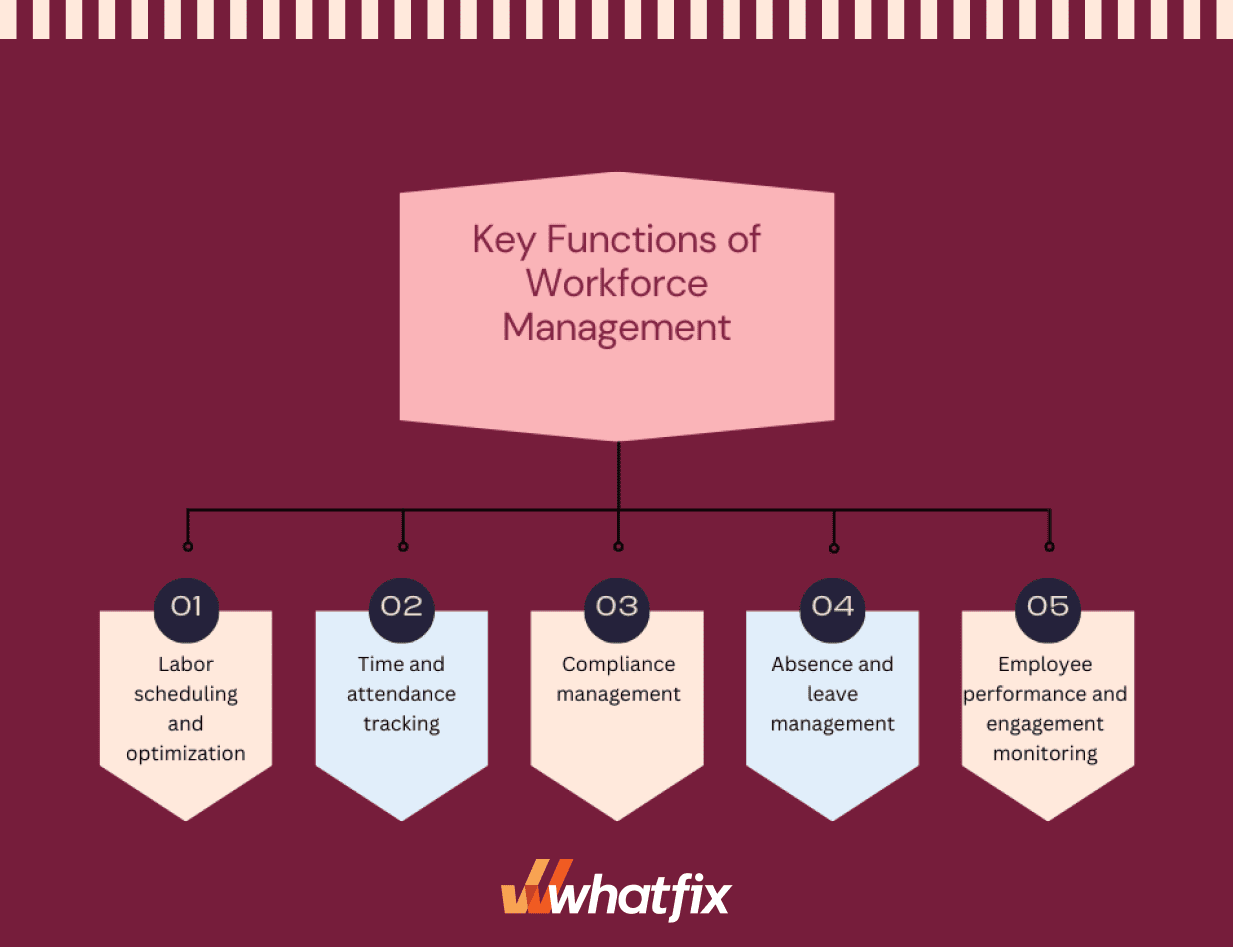
\includegraphics[width=1\linewidth]{Workforce.png}
    \caption{Overview of workforce management features}
    \label{fig:workflowFeatures}
\end{figure}.

\section{Theoretical Frameworks in Software Architecture}
\subsection{Constraint Satisfaction Problems in Automated Scheduling}

The foundation of modern algorithmic scheduling lies in the field of artificial intelligence and operations research, specifically within the domain of Constraint Satisfaction Problems (CSP). A CSP is defined mathematically by a set of variables (e.g., available work shifts), a domain of values for each variable (e.g., the pool of available employees), and a set of constraints that restrict the allowable combinations of values. \cite{Meseguer1989}

In workforce management, these constraints are categorized as either hard or soft. Hard constraints are non-negotiable boundaries, such as legal maximum weekly working hours or mandatory rest periods between shifts. Soft constraints represent operational preferences, such as an employee's desire to work morning shifts or a manager's preference to balance out the working hours for each employee. The theoretical challenge—and computational complexity—of automated scheduling systems lies in designing algorithms capable of navigating these multi-dimensional constraints to find an optimal, legally compliant assignment without requiring exponential computational time.

\subsection{Multi-Tenant Software-as-a-Service (SaaS) Paradigms}
 
The architectural shift from locally hosted, single-tenant applications to a future cloud-based Software-as-a-Service (SaaS) platforms requires robust Multi-Tenancy models. Multi-tenancy refers to a software architecture in which a single instance of an application serves multiple distinct user groups, or "tenants."\cite{MultiTenantSaaS}

From a theoretical standpoint, multi-tenant data architecture generally falls into three categories: isolated databases, isolated schemas within a shared database, or a shared database with shared schemas. Modern SaaS platforms frequently employ the latter for its scalability and cost-efficiency. However, this approach necessitates strict programmatic barriers—often termed Context-Aware Data Isolation—to ensure that a tenant (e.g., an independent store branch) cannot access or manipulate the data of another tenant, requiring security logic to be deeply embedded into the application's data persistence layer.

\begin{figure}[!h]
    \centering
    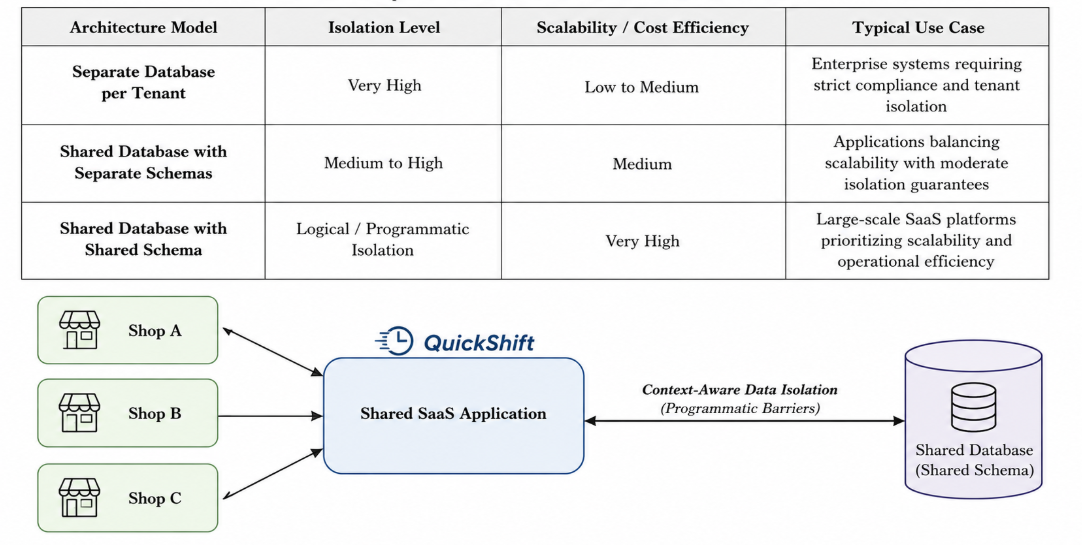
\includegraphics[width=1\linewidth]{SharedSchema.png}
    \caption{Shared Database Schema and table}
    \label{fig:placeholder}
\end{figure}

\subsection{Advanced Role-Based Access Control (RBAC) and Stateless Authentication}

To support secure multi-tenancy, access control mechanisms have evolved significantly. Traditional, stateful session-based authentication has largely been superseded by stateless protocols utilizing JSON Web Tokens (JWT).

While basic Role-Based Access Control (RBAC) relies on checking a user's assigned role against a requested endpoint (e.g., validating if a user has "ADMIN" privileges), enterprise-grade systems require Layer 2 Data-Level RBAC. In this theoretical model, access control is not merely a gatekeeper at the application's edge; rather, the authentication identity is injected directly into the data querying process. This ensures that data retrieval is dynamically scoped to the user's specific organizational context, rendering unauthorized horizontal data access architecturally impossible.\cite{RBAC1}

\section{Market Analysis of Workforce Management Solutions}
\subsection{Global Market Dynamics and Growth Indicators}

The demand for intelligent workforce management solutions is experiencing rapid and sustained growth, driven by increasing emphasis on operational efficiency and labor compliance. According to recent industry projections, the global Employee Scheduling and Shift Planning Software market is expected to grow from approximately USD 1.89 billion in 2024 to nearly USD 3.94 billion by 2032, representing a Compound Annual Growth Rate (CAGR) of 9.6\%. \cite{SchedulingMarket2024}.\begin{equation}
\text{CAGR} = \left( \frac{V_{final}}{V_{begin}} \right)^{\frac{1}{t}} - 1
\end{equation}
This expansion is largely fueled by the transition of Small and Medium Enterprises (SMEs) away from manual spreadsheet-based scheduling toward centralized, cloud-based Software-as-a-Service (SaaS) platforms that provide automated workforce optimization and compliance management.

\begin{figure}[H]
    \centering
    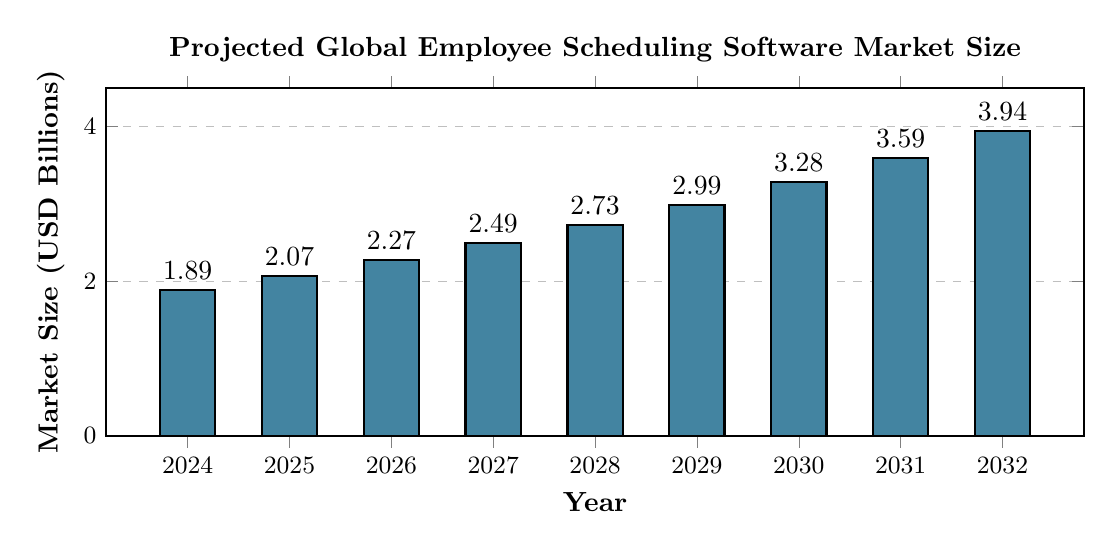
\begin{tikzpicture}
        \begin{axis}[
            ybar,
            bar width=20pt,
            width=14cm,
            height=6cm,
            title={\textbf{Projected Global Employee Scheduling Software Market Size}},
            xlabel={Year},
            ylabel={Market Size (USD Billions)},
            symbolic x coords={2024, 2025, 2026, 2027, 2028, 2029, 2030, 2031, 2032},
            xtick=data,
            nodes near coords, % Displays the values on top of the bars
            nodes near coords align={vertical},
            ymin=0, ymax=4.5,
            enlarge x limits=0.1,
            % Styling the chart for a professional thesis look
            axis line style={thick},
            tick label style={font=\small},
            label style={font=\normalsize\bfseries},
            ymajorgrids=true,
            grid style=dashed,
        ]
            % Data calculated using: 1.89 * (1 + 0.096)^(Year - 2024)
            \addplot[fill=cyan!60!black, draw=black, thick] coordinates {
                (2024, 1.89)
                (2025, 2.07)
                (2026, 2.27)
                (2027, 2.49)
                (2028, 2.73)
                (2029, 2.99)
                (2030, 3.28)
                (2031, 3.59)
                (2032, 3.94)
            };
        \end{axis}
    \end{tikzpicture}
    \caption{Projected market growth from 2024 to 2032.}
    \label{fig:market_growth_projection}
\end{figure}

\subsection{Ecosystem of Leading Competitors}

The current commercial landscape is dominated by several large-scale SaaS providers, each targeting broad demographics of shift-based industries:

\begin{itemize}
    \item \textbf{Deputy:} Recognized as a market leader, Deputy provides a comprehensive suite of workforce management tools. Its core strengths lie in automated scheduling based on robust historical data and extensive integrations with third-party payroll systems. It is primarily built for medium-to-large enterprises in retail and hospitality \cite{Deputy}.
    
    \item \textbf{ShiftIn:} Targeted at small and medium Romanian businesses, ShiftIn offers closer maintenance support with more customization for a monthly, subscription fee. \cite{ShiftIn}.

    \item \textbf {Homebase:} Targeted more aggressively at small businesses, Homebase offers an accessible entry point with core features like drag-and-drop scheduling, basic team communication, and time-tracking. \cite{Homebase}
    
    \item \textbf{When I Work:} This platform differentiates itself through strong mobile-first employee self-service capabilities, allowing workers to easily trade shifts, request time off, and manage their availability directly from their smartphones. \cite{WhenIWork}

    
\end{itemize}

\subsection{Identifying the Architectural and Functional Gap}

Despite the maturity of the previously mentioned platforms, a critical analysis reveals significant structural gaps, particularly regarding niche adaptability and proactive automation for SMEs.

First, leading platforms operate on a "One-Size-Fits-All" paradigm. To accommodate every possible industry—from healthcare to construction. Their core employee models are overly generalized. Businesses requiring highly specific, localized HR metrics (such as unique holiday recovery tracking or strict contract-type delineations like "Part-Time 4H vs. 6H") often find these tools either incapable of enforcing these rules or requiring prohibitively expensive "Enterprise" tier customizations.

Furthermore, while current systems excel at reactive scheduling—such as allowing an employee to drop a shift and notifying a manager to manually find a replacement—there is a distinct lack of proactive algorithmic automation. Existing platforms either rely on manual managerial intervention to resolve last-minute staffing shortages, or assign the shift just to the first eligible worker.s QuickShift addresses this limitation through its \texttt{findBestCandidate} function, which automatically evaluates labor constraints and individual preferences to identify and assign the optimal replacement worker, rather than merely the first available one. 

\begin{figure}[!h]
    \centering
    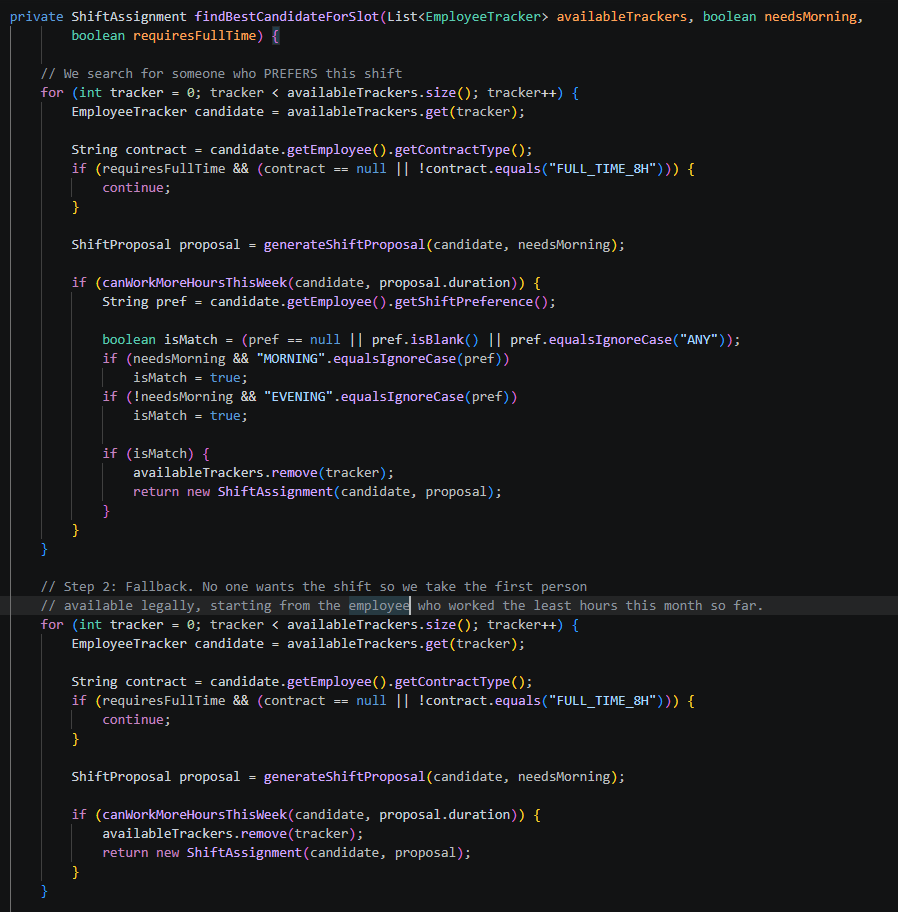
\includegraphics[width=0.7\linewidth]{findBestCandidate.png}
    \caption{findBestCandidate function}
    \label{fig:placeholder}
\end{figure}

This identified gap between generalized, reactive software and the need for highly specific, automated operational continuity forms the foundational premise for the architectural solutions proposed in the subsequent chapters.
\chapter{System Architecture}
\label{chap:ch3}

\par The architecture of this workforce management application was designed following modern, enterprise-grade software engineering principles. To ensure high cohesion, loose coupling, and horizontal scalability, the system adopts a decoupled Client-Server Architecture.

The application is strictly divided \textbf{into 4 distinct tiers}: a relational Data Persistence layer, a robust Application layer driven by an Inversion of Control (IoC) container, a secure stateless Integration layer, and a component-based Presentation layer. At the core of the Application layer sits a \textbf{custom heuristic solver}, designed specifically to address the complex \textbf{Constraint Satisfaction Problem (CSP) of generating Labor Code-compliant shift schedules}. By separating these concerns, the architecture ensures that the algorithmic complexity of the backend is entirely abstracted away from the end-user, resulting in a secure, responsive, and easily maintainable system.

\begin{figure}[!h]
    \centering
    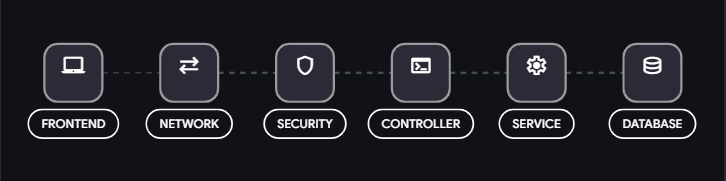
\includegraphics[width=1\linewidth]{Diagrama.png}
    \caption{Overview of data flow}
    \label{fig:dataFlow}
\end{figure}


\section{Technological Stack Overview}
\label{sec:ch3sec1}

\par The technological stack overview represents a comprehensive overview of the selected technological stack, detailing the rationale behind each architectural decision. Rather than relying on a tightly coupled monolithic structure, this system utilizes a modern, decentralized stack. Each framework and tool was deliberately chosen for its ability to fulfill specific architectural requirements, ranging from secure data persistence to complex algorithmic processing and dynamic user interaction.


\subsection{Data persistence : Microsoft SQL Server}
\label{subsec:ch3sec1subsec1}

\par For the underlying relational database tier, Microsoft SQL Server was selected. As a Tier-1 enterprise Relational Database Management System, it provides strict ACID (Atomicity, Consistency, Isolation, Durability) compliance, ensuring absolute data integrity for critical domain entities such as user credentials, store configurations, and generated labor shifts. Its seamless integration with SQL Server Management Studio (SSMS) also facilitates efficient database administration, querying, and schema verification during the application lifecycle. Moreover, the ability to easily integrate this DB with the best clouding hosts available (AWS and Microsoft Azure) makes it the best option available. \cite{pass2025}

\subsection{Application logic: Java + Spring Boot}
\label{subsec:ch3sec1subsec2}

\par The core backend logic, including the custom heuristic scheduling algorithm, is implemented using Java 17 and the Spring Boot 3 framework. Spring Boot was chosen primarily for its powerful Inversion of Control (IoC) container, which drastically reduces structural boilerplate and manages object lifecycles through Dependency Injection. It also provides the Spring Security module, which is broken down in the Security subsection. Furthermore, the integration of Spring Data JPA abstracts complex SQL queries into a highly efficient Object-Relational Mapping (ORM) layer via Hibernate, allowing the application layer to interact with the database efficiently and safely, while keeping the code clean and modern. Moreover, Java + Spring Boot is arguably the most used combination of tools worldwide for these types of application, therefore automatically granting multiple quality references and documents to learn and debug from, should there be any problems whatsoever.\cite{GuideOnJavaAndSpringBoot}

\subsection{Integration and security: REST and JWT}
\label{subsec:ch3sec1subsec3}

\par To ensure complete decoupling between client and server, communication is handled exclusively via a \textbf{RESTful API}. The API is secured with a stateless JWT-based pipeline in Spring Security, so the server does not keep session state in memory. On each request, the token is validated cryptographically to recover the user identity (subject), and the backend loads the user from the database via \texttt{UserDetailsService} to obtain the current roles/authorities for RBAC enforcement. This keeps the system stateless while still relying on per-request database lookups for user role resolution. In this design, role changes or user deactivation take effect immediately, because each request revalidates the user against the database before authorization is granted. \cite{mario2025hybrid}

\subsection{Presentation layer: React}
\label{subsec:ch3sec1subsec4}
\par The frontend presentation layer was developed using React, a component-based JavaScript library. React was selected specifically for its Virtual DOM architecture, which enables highly efficient, localized rendering of complex user interfaces. This is an essential requirement for this application, as rendering interactive, multi-dimensional monthly shift schedules requires rapid UI updates without reloading the entire web page. The component-driven approach also ensures high code reusability and maintainability across the application's administrative dashboards.

\begin{figure}[!h]
    \centering
    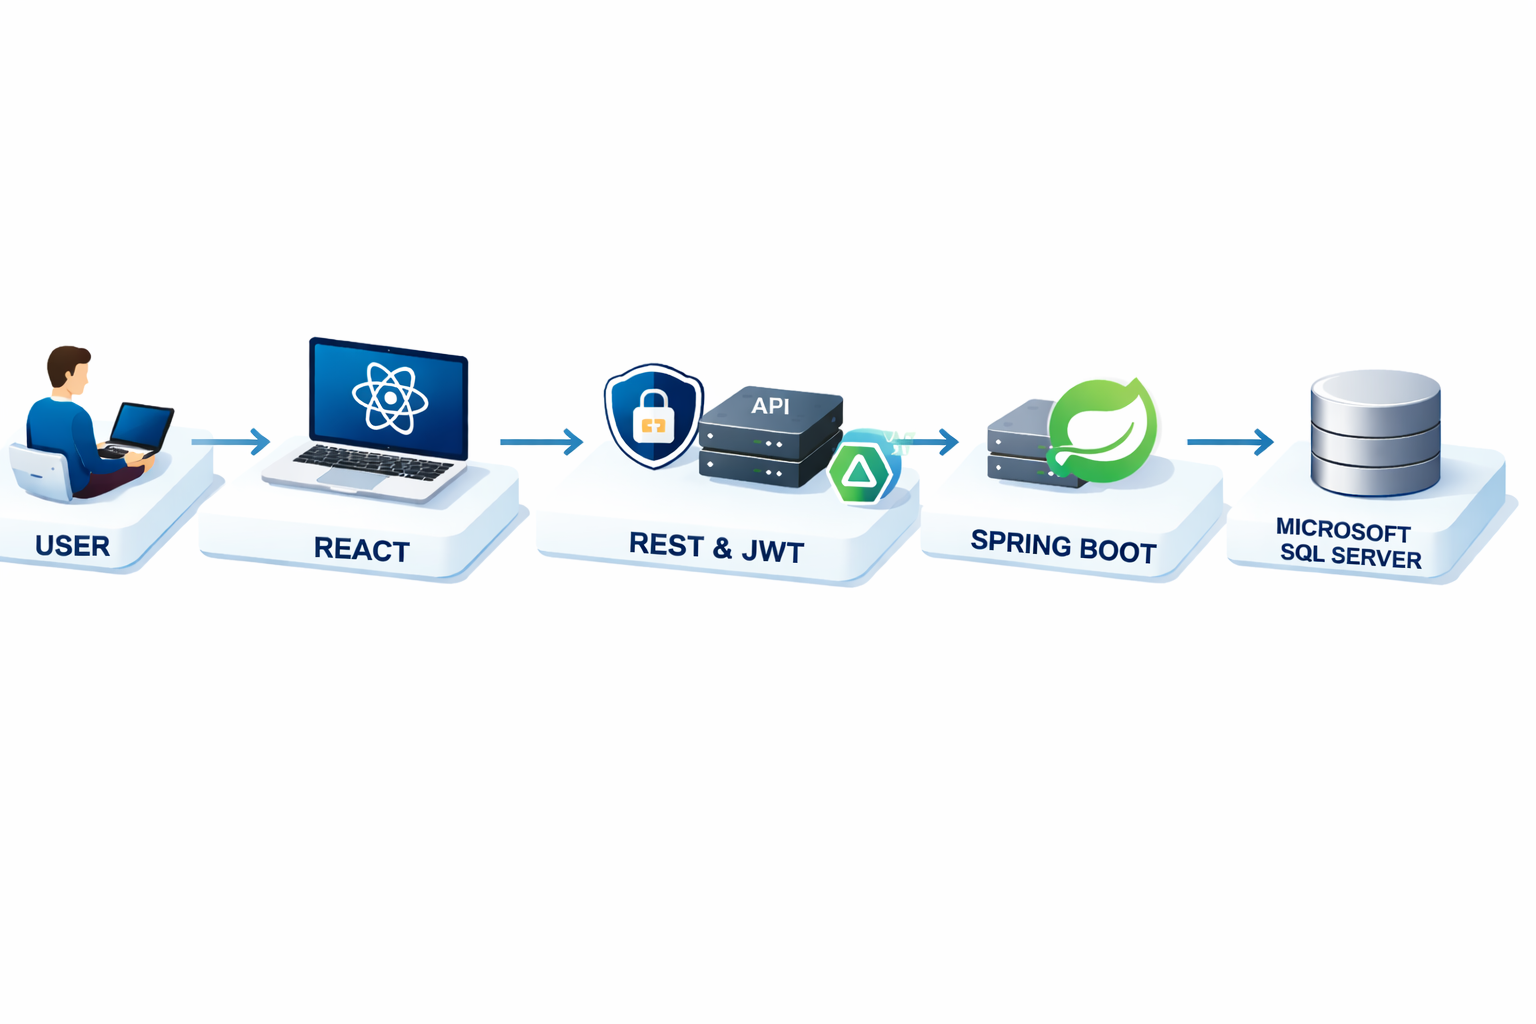
\includegraphics[width=1\linewidth]{DiagramTechStack.png}
    \caption{Technology Stack High Overview}
    \label{fig:tech_stack}
\end{figure}

\section{Practical Application of the System Architecture}
\label{sec:ch3sec2}

\par This section delves into the practical application of the technologies that form the backbone of the workforce management application. While the previous section justified the choice of each technology, this section focuses on their real-world implementation and interaction within the system.

\subsection{Database layer: Data integrity and accessibility}
\label{subsec:ch3sec2subsec1}

\par The database layer, implemented using Microsoft SQL Server, is structured to ensure data integrity and accessibility. Critical entities such as user credentials, labor shifts, and store configurations are stored in normalized tables to minimize redundancy and maintain consistency. The database schema is designed to enforce relationships and constraints, ensuring that the data remains reliable and secure.

\par The integration with Spring Data JPA allows the application layer to interact with the database through a high-level abstraction. This eliminates the need for manual SQL queries, as the ORM layer translates Java objects into database operations. For example, user registration and authentication processes involve creating and querying user records, which are seamlessly handled by the repository layer.

\subsection{Application layer: Business logic implementation}
\label{subsec:ch3sec2subsec2}

\par The application layer is the core of the system, where the business logic is implemented. Using Java 17 and Spring Boot 3, this layer manages operations such as user authentication, shift scheduling, and data validation. The custom heuristic scheduling algorithm, designed to solve the Constraint Satisfaction Problem (CSP), is implemented here to generate Labor Code-compliant shift schedules.

\par Dependency Injection, facilitated by Spring Boot's IoC container, ensures that components such as the `AuthenticationService` and `JwtService` are loosely coupled and easily testable. For instance, the `AuthenticationService` handles user registration and login by validating input, encoding passwords, and generating JWT tokens for secure communication.

\begin{figure}[H]
    \centering

    \begin{subfigure}{\linewidth}
        \centering
        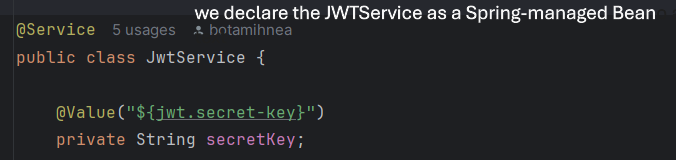
\includegraphics[width=0.65\linewidth,
                        height=0.10\textheight,
                        keepaspectratio]
                        {CodeSnippet-JwtService-Edit.PNG}
        \caption{JwtService Initialization}
    \end{subfigure}

    \vspace{0.2em}

    \begin{subfigure}{\linewidth}
        \centering
        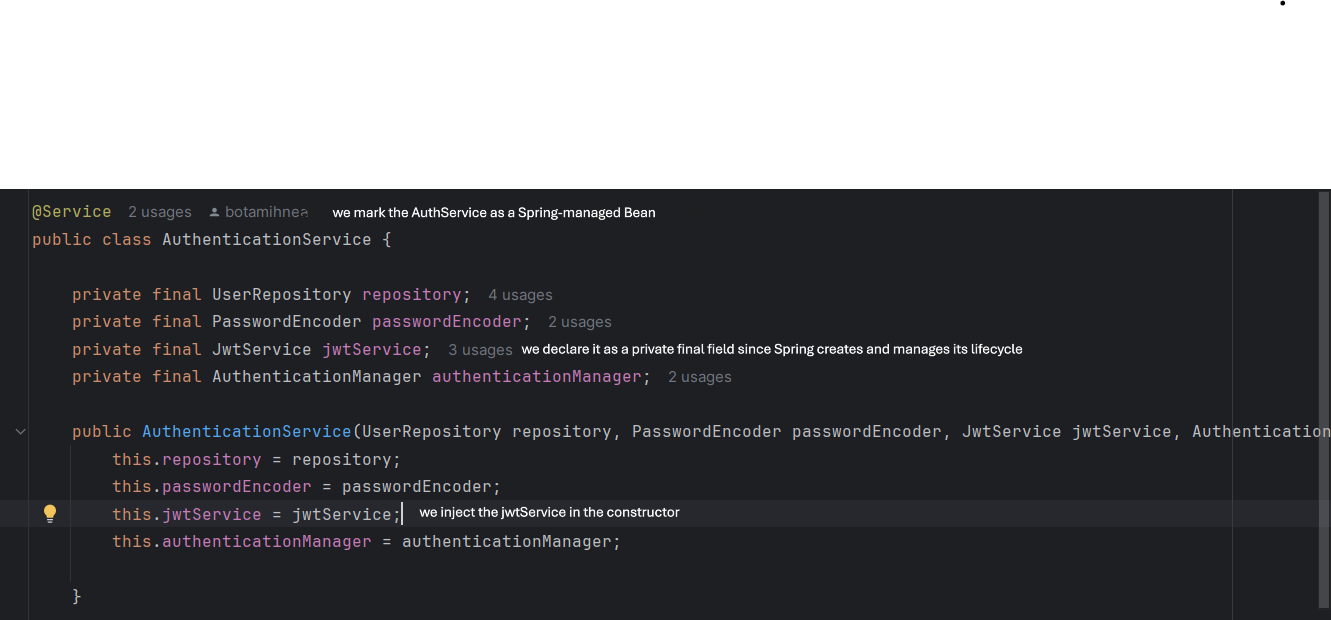
\includegraphics[
            width=0.80\linewidth,
            height=0.18\textheight,
            trim=20 20 20 20,
            clip]{CodeSnippet-AuthenticationService-Edited.PNG}
        \caption{AuthenticationService Initialization}
    \end{subfigure}

    \caption{Service initialization code snippets}
    \label{serviceInitCodeSnippets}
\end{figure}

\subsection{Integration layer: Secure communication}
\label{subsec:ch3sec2subsec3}

\par The secure bridge between the React frontend and the Spring Boot backend is facilitated by a custom Spring Security filter chain. Rather than relying on default session management, the system intercepts incoming HTTP requests using a custom \textbf{JwtAuthenticationFilter}.

\par When a client attempts to access a protected endpoint, such as the shift generation API, this filter extracts the Bearer token from the \textbf{Authorization} header. It then utilizes the \textbf{JwtService} to cryptographically verify the token's signature and expiration date. If valid, the user's role (e.g., \textbf{MANAGER}) is extracted from the database based on the user's identifier(email) from the token payload and injected into the \textbf{SecurityContextHolder}. This implementation allows the \textbf{SecurityConfig} class to seamlessly enforce Role-Based Access Control (RBAC) at the endpoint level, immediately rejecting unauthorized traffic with an HTTP 403 Forbidden status before it ever reaches the controller logic.

\subsection{Frontend layer: Dynamic user interaction}
\label{subsec:ch3sec2subsec4}

\par The frontend, developed using React, provides a dynamic and interactive user experience. By leveraging React's Virtual DOM, the application efficiently updates the user interface in response to user actions. For instance, when a user generates a shift schedule, the frontend sends a request to the backend API and updates the displayed schedule based on the response.

\par The component-based architecture of React ensures that the user interface is modular and maintainable. Each component is responsible for a specific part of the interface, such as the login form or the schedule viewer, making it easier to manage and extend the application.

\subsection{End-to-End workflow}
\label{subsec:ch3sec2subsec5}

\par The end-to-end workflow begins with the user interacting with the React-based frontend. User actions, such as submitting a login form, trigger HTTP requests to the backend API. The backend processes these requests by validating the JWT token, executing the necessary business logic, and interacting with the database as needed. The results are then returned to the frontend, which updates the user interface accordingly.

\par This workflow demonstrates the seamless integration of the chosen technologies, with each layer performing its role independently while contributing to the overall functionality of the system. By adhering to modern software engineering principles, the application achieves a balance between scalability and maintainability.



\chapter{Algorithm Implementation and Operational Workflows}
\label{chap:ch4}

\par This chapter describes in detail the concrete implementation of every major operational flow in the QuickShift system. Beyond the core scheduling engine, the platform manages a full lifecycle of workforce events: leave requests submitted by employees, absence reports that trigger automated replacement searches, manual corrections made by managers, and the complete notification loop that connects all participants. Each of these workflows is underpinned by the same constraint-satisfaction principles used in the scheduler, ensuring behavioral consistency across the system.

%===========================================================
\section{Automated Schedule Generation}
\label{sec:automated_schedule_generation}
%===========================================================

\subsection{Input data and preprocessing}
\par Every scheduling run begins with a data ingestion step. The backend reads a structured Excel file that contains one row per working day, carrying at minimum a date, a projected daily sales figure, and a boolean flag indicating whether a merchandise reception is expected on that day. The reading is performed by a dedicated \texttt{CsvReaderService} and the output is a typed list of \texttt{DayForecastDto} objects, each encapsulating the complete context needed for a single day of scheduling.

\par The target month is resolved to the next calendar month automatically. This design keeps the scheduling endpoint simple for the most common use case while still supporting the Leave Request functionality, by only allowing employees to request leave with at least 1 month prior. In this way we make sure that the schedule does not shift as much with only a few days before the month's beginning, and therefore it does not confuse the employees with massive changes on short notice.

\par For deployments serving multiple stores, the forecast Excel can be organized into named sheets, each corresponding to a store. The backend accepts an optional store identifier which is translated into a sheet name via the \texttt{Store} entity. If no matching sheet is found or the resulting row set for the requested month is empty, the generation is aborted early and a clear error is returned to the caller. This prevents silently producing an empty or partial schedule when input data is missing.

\subsection{Schedule generation pipeline}
\par The overall generation flow is structured as a deterministic pipeline that processes the forecast list sequentially. Before computing any new assignments, the system retrieves all existing shifts for the target month and store from the database. If any exist, they are removed together with their linked absence requests and replacement offers, ensuring that the regenerated schedule is always internally consistent and does not contain residual data from a previous run.

\par This delete-before-generate strategy is a deliberate architectural choice. An alternative approach would be to compute a diff between the old and new schedules and apply only the changes. While that would produce smaller database operations, it introduces significant complexity in handling the intermediate states of absence requests and replacement chains that may reference old shifts. The chosen approach trades a slightly larger write at generation time for a dramatically simpler consistency model, which is more appropriate for the operational scale of the target deployment.

\par After the cleanup phase, employee trackers are initialized for all employees in scope, and the algorithm iterates day by day through the forecast list. At the end of the loop, all produced shift objects are persisted in bulk using a single \texttt{saveAll} call, which keeps the transaction boundary short and avoids partial writes.

\subsection{The Constraint Model}
\par The solver enforces two categories of constraints. Hard constraints represent legal or operational limits that must hold unconditionally for any produced schedule:

\begin{itemize}
    \item \textbf{Maximum consecutive working days}: no employee may work more than five days in a row. Once this limit is reached, the employee is excluded from candidate selection until a day off is registered.
    \item \textbf{12-hour back-to-back prohibition}: an employee who worked a 12-hour shift on the previous day is excluded from the following day's assignment, regardless of weekly hour accumulation.
    \item \textbf{Weekly hour caps}: the maximum number of hours assignable in a single calendar week depends on contract type. Full-time employees (8-hour contracts) may not exceed 40 hours per week; employees on a 6-hour part-time contract are capped at 30 hours; employees on a 4-hour contract are capped at 20 hours per week.
    \item \textbf{Approved leave}: employees with an approved leave request covering the target day are completely excluded from candidate selection for that day.
\end{itemize}

\par Soft constraints guide candidate ranking when multiple legal candidates exist. The primary soft rule is shift preference: employees who have declared a preference for morning or evening shifts are ranked above equally eligible candidates with a different preference or no declared preference. The secondary soft rule is monthly hour balance: among candidates with the same preference score, the one with the fewest accumulated hours in the current month is preferred. Together, these two soft rules produce schedules that are both preference-aligned and balanced without requiring a dedicated optimization pass. Technically speaking, this is the \textbf{true game-changer for QuickShift}. While other tools available on the market design basic end-to-end shifts that only take into account the hard constraints, this application truly takes into consideration what the employee prefers, therefore significantly raising the quality of work produced. All this is done in parallel with the forecast functionality, achieving a balance between the quality of life and productivity for the employee.

\subsection{Coverage scaling from forecast signals}
\par The default staffing target is one employee per time window (morning and evening), for a daily total of two employees.

Several business rules are used to adjust staffing requirements. First, the weekend effect accounts for the fact that Saturday and Sunday are inherently high-traffic days in retail. Therefore, the minimum staffing level for both the morning and evening slots is raised to two employees, resulting in a daily total of four employees.

Similarly, on a reception day, when a merchandise shipment is expected, additional staff are required to unload and process stock. As a result, the minimum staffing level for both slots is also raised to two employees.

The day before reception is subject to the same elevated staffing requirements because preparation work must be carried out in anticipation of the incoming shipment.

Sales projections also influence staffing levels. Under the big sales threshold rule, if the projected daily sales exceed a configurable threshold (currently set to 2,000 monetary units), one additional employee is assigned to the evening slot to accommodate increased customer traffic during peak afternoon hours.

Finally, the massive sales threshold rule applies when projected sales exceed a higher threshold (currently 5,000 monetary units). In this case, an additional employee is assigned to the morning slot as well, reflecting the needs of exceptional commercial events such as national holidays or promotional campaigns.

\par These thresholds are defined as instance fields in the scheduling service and can be adjusted without modifying the algorithm logic. The design makes the coverage model transparent and tunable by someone with domain knowledge, without requiring code changes.

\subsection{Heuristic solver and the employee tracker}
\par The solver is built on a greedy heuristic enhanced by a stateful per-employee tracking structure called \texttt{EmployeeTracker}. Each tracker wraps an \texttt{Employee} entity and maintains three pieces of mutable state:

\begin{figure}[h!]
    \centering
    \begin{tikzpicture}[
        node distance=1.5cm and 1.5cm,
        mainbox/.style={rectangle, draw=blue!70, thick, fill=blue!5, text width=3.5cm, align=center, rounded corners=1ex, minimum height=1.2cm, font=\sffamily\bfseries},
        metricbox/.style={rectangle, draw=black!70, thick, fill=gray!5, text width=5cm, align=left, rounded corners=1ex, minimum height=1cm, font=\sffamily\small},
        limitbox/.style={rectangle, draw=red!60, thick, fill=red!5, text width=3.5cm, align=left, rounded corners=1ex, minimum height=0.6cm, font=\sffamily\footnotesize},
        arrow/.style={thick, ->, >=stealth, draw=black!70},
        dashedarrow/.style={thick, ->, >=stealth, draw=red!70, dashed}
    ]

    % Main Engine Node
    \node (engine) [mainbox] {Algorithm \\ Tracking Engine};

    % Metric Nodes
    \node (weekly) [metricbox, right=1.5cm of engine] {\textbf{Weekly Hours} \\ Cumulative ISO week total};
    \node (monthly) [metricbox, above=0.8cm of weekly] {\textbf{Monthly Hours} \\ Cumulative month total};
    \node (consecutive) [metricbox, below=0.8cm of weekly] {\textbf{Consecutive Days} \\ Unbroken sequence counter};

    % Reset/Limit Nodes
    \node (rmonthly) [limitbox, right=1cm of monthly] {Reset: 1st of Month};
    \node (rweekly) [limitbox, right=1cm of weekly] {Reset: Every Monday};
    \node (rconsecutive) [limitbox, right=1cm of consecutive] {Limit: 5 Days \\ Reset: Day-Off};

    % Arrows from Engine to Metrics
    \draw [arrow] (engine.east) -- ++(0.5,0) |- (monthly.west);
    \draw [arrow] (engine.east) -- (weekly.west);
    \draw [arrow] (engine.east) -- ++(0.5,0) |- (consecutive.west);

    % Arrows from Metrics to Limits
    \draw [dashedarrow] (monthly.east) -- (rmonthly.west);
    \draw [dashedarrow] (weekly.east) -- (rweekly.west);
    \draw [dashedarrow] (consecutive.east) -- (rconsecutive.west);

    \end{tikzpicture}
    \caption{Internal metric tracking and constraint triggers utilized by the scheduling algorithm.}
    \label{fig:algorithm_tracking}
\end{figure}

\par On each day, the solver computes the total number of employee slots to fill and iterates through them in order. For each slot it determines whether the next assignment must be a morning or evening shift, and whether it is the first assignment of that slot (which requires a full-time employee to maintain service quality). Candidates are sorted by least monthly hours before preference matching is attempted, so the greedy selection naturally distributes hours across the team over the course of the month.

\par The selection itself proceeds in two passes. The first pass looks only at candidates whose declared preference matches the required slot. If such a candidate exists and satisfies all hard constraints, they are selected immediately. If the first pass finds no match, a second fallback pass selects the legally available candidate with the smallest amount of hours worked in that specific month, regardless of preference. This two-pass design avoids sacrificing coverage when no preferred candidate is available, while still honoring preferences whenever they do not conflict with operational needs.

\subsection{Shift proposal generation and contract mapping}
\par Once a candidate is selected, the system generates a concrete shift proposal based on their contract type and the required time window. The mapping is as follows:

\begin{table}[h]
\centering
\caption{Shift mapping by contract type and slot}
\begin{tabular}{|l|l|l|}
\hline
\textbf{Contract Type} & \textbf{Morning Slot} & \textbf{Evening Slot} \\ \hline
\texttt{FULL\_TIME\_8H} 
& \texttt{SHIFT\_1\_10\_18} (10:00--18:00) 
& \texttt{SHIFT\_2\_14\_22} (14:00--22:00) \\ \hline

\texttt{PART\_TIME\_6H} 
& \texttt{PART\_TIME\_10\_16} 
& \texttt{PART\_TIME\_16\_22} \\ \hline

\texttt{PART\_TIME\_4H} 
& \texttt{PART\_TIME\_10\_14} 
& \texttt{PART\_TIME\_16\_20} \\ \hline
\end{tabular}
\label{tab:shift_mapping}
\end{table}

\par Each proposal carries the shift type string, the duration in hours, and a boolean indicating whether it falls in the morning window. The duration is used immediately for the weekly hour check before the candidate is accepted, preventing over-assignment at the point of selection rather than as a post-processing correction.

%===========================================================
\section{Absence and Replacement Workflows}
\label{sec:absence_and_replacement_workflows}
%===========================================================

\subsection{The absence reporting flow}
\par Employees frequently need to report that they cannot attend a scheduled shift on short notice. The system provides a structured absence reporting mechanism that initiates a formal workflow rather than relying on informal communication between the employee and the manager.

\par When an employee submits an absence report through the frontend, the backend validates several preconditions before accepting it:

\begin{itemize}

    \item The shift must belong to the requesting employee (ownership verification).

    \item The shift date must be strictly in the future — past shifts cannot be reported.

    \item The shift must be in a reportable state: both \texttt{SCHEDULED} and \texttt{REPLACEMENT} shifts are eligible, but a shift that has already been marked \texttt{ABSENT} or is in another terminal state is rejected.

    \item There must not already be a pending absence request for the same shift, preventing duplicate submissions.

\end{itemize} 


\par If all checks pass, an \texttt{AbsenceRequest} entity is persisted with status \texttt{PENDING}, and a notification is sent to the store manager. The notification message follows a structured format prefixed with \texttt{[ABSENCE REQUEST]}, which allows the frontend to identify the notification type and render the appropriate action control. The notification carries a reference to the absence request ID, linking the notification to the workflow object without duplicating data.

\subsection{Manager acknowledgment and the replacement algorithm}
\par Upon receiving an absence notification, the manager can acknowledge the request directly from the notifications page. Acknowledgment triggers a multi-step process:

\vspace{1.5em}
\begin{figure}[!h]
    \centering
    \begin{tikzpicture}[
        node distance=0.8cm,
        startbox/.style={rectangle, draw=blue!70, thick, fill=blue!5, text width=7.5cm, align=center, rounded corners=1ex, minimum height=0.8cm, font=\sffamily\bfseries},
        actionbox/.style={rectangle, draw=black!70, thick, fill=gray!5, text width=7.5cm, align=left, rounded corners=1ex, minimum height=0.9cm, font=\sffamily\small},
        decisionbox/.style={diamond, aspect=2.5, draw=orange!70, thick, fill=orange!5, text width=4.5cm, align=center, font=\sffamily\small\bfseries},
        deductbox/.style={rectangle, draw=red!70, thick, fill=red!5, text width=4cm, align=center, rounded corners=1ex, minimum height=0.8cm, font=\sffamily\small},
        enginebox/.style={rectangle, draw=purple!70, thick, fill=purple!5, text width=7.5cm, align=center, rounded corners=1ex, minimum height=0.9cm, font=\sffamily\bfseries},
        arrow/.style={thick, ->, >=stealth, draw=black!70}
    ]

    % Nodes
    \node (start) [startbox] {Absence Request Approved};
    
    \node (step1) [actionbox, below=0.8cm of start] {\textbf{1. State Update} \\ Original shift marked as \texttt{ABSENT}. Visible on public calendar.};
    
    \node (step2) [decisionbox, below=0.8cm of step1] {Was it a regular \\ (non-replacement) shift?};
    
    \node (deduct) [deductbox, right=1cm of step2] {\textbf{2. Leave Deduction} \\ Decrement balance by 1};
    
    \node (step3) [enginebox, below=1cm of step2] {\textbf{3. Replacement Finder Engine} \\ System searches for the optimal available substitute};

    % Arrows
    \draw [arrow] (start) -- (step1);
    \draw [arrow] (step1) -- (step2);
    
    % Decision branch: YES
    \draw [arrow] (step2.east) -- node[above, font=\sffamily\footnotesize] {Yes} (deduct.west);
    \draw [arrow] (deduct.south) |- (step3.east);
    
    % Decision branch: NO
    \draw [arrow] (step2.south) -- node[right, font=\sffamily\footnotesize] {No} (step3.north);

    \end{tikzpicture}
    \caption{Automated system workflow triggered upon reporting a shift absence.}
    \label{fig:absence_processing_workflow}
\end{figure}
\vspace{1.5em}

\par The replacement finder reconstructs the full scheduling state for the target month before making its selection. It loads all shifts for the store from the beginning of the month up to and including the absence date, then replays them day by day through \texttt{EmployeeTracker} instances. This replay ensures that the replacement search respects the same constraints as the original scheduler: weekly hours are tracked correctly across ISO week boundaries, consecutive day counts are accurate, and no candidate is selected who would violate a hard constraint as a result of the replacement assignment.

\par After the replay, the finder applies the following eligibility filters to the candidates:

\vspace{1.5em}
\begin{table}[h!]
    \centering
    \caption{Algorithmic constraints evaluated by the replacement finder engine.}
    \renewcommand{\arraystretch}{1.5}
    \begin{tabular}{|l|p{4.5cm}|p{6cm}|}
        \hline
        \textbf{Domain} & \textbf{Constraint Metric} & \textbf{Algorithmic Application} \\ \hline
        \multirow{2}{*}{\textbf{Availability}} & Not Already Scheduled & Rejects candidates who already possess an assigned shift on the target date. \\ \cline{2-3}
        & Not on Approved Leave & Cross-references the leave database; excludes employees on official vacation. \\ \hline
        \multirow{2}{*}{\textbf{Fatigue \& Rest}} & Consecutive Days Limit & Evaluates trailing schedule; candidate must have worked $< 5$ unbroken days. \\ \cline{2-3}
        & 12-Hour Rest Mandate & Excludes candidates who worked a 12-hour shift immediately preceding the target date. \\ \hline
        \multirow{2}{*}{\textbf{Contractual}} & Weekly Hour Cap & The replacement shift's duration must not exceed the candidate's legal weekly maximum. \\ \cline{2-3}
        & Contract Compatibility & Full-Time employees bypass duration checks. Part-Time employees are strictly matched to slots equaling their contractual daily hours. \\ \hline
    \end{tabular}
    \label{tab:replacement_constraints}
\end{table}
\vspace{1.5em}

\par Eligible candidates are sorted by a two-key comparator. The primary key is a preference score: candidates whose declared shift preference matches the morning or evening character of the absent shift receive a score of 0 (best); candidates with no preference or the \texttt{ANY} designation receive a score of 1; candidates whose preference is opposite to the required slot receive a score of 2 (last resort). The secondary key is the accumulated hours worked in the current month, ensuring that among equally preferred candidates the one with the lighter workload is selected first. This mirrors the fairness logic of the main scheduler.

\par Previously declined employees are automatically excluded from consideration in subsequent attempts. The system tracks all replacement offers linked to a given absence request and builds an exclusion set before invoking the finder, so the same employee is never asked twice for the same absence.

\subsection{The replacement offer flow}
\par When a suitable replacement is found, the system does not immediately assign the shift. Instead, it creates a \texttt{ReplacementOffer} entity linking the absence request, the candidate employee, and the shift details. This offer is then presented to the candidate employee through a notification, allowing them to accept or decline the extra assignment voluntarily.

\par The notification sent to the employee uses the prefix \texttt{[REPLACEMENT OFFER]} and carries the replacement offer ID as a reference, which the frontend uses to render the accept/decline action buttons. A second notification with the same prefix is sent to the manager to confirm that an offer has been dispatched. The absence request status is updated to \texttt{PENDING\_REPLACEMENT} to reflect that the workflow is in progress.

\subsubsection*{Offer acceptance}
\par When the employee accepts the offer, the backend performs the following steps atomically within a single transaction:

\begin{itemize}
    \item A new \texttt{Shift} entity is created with status \texttt{REPLACEMENT} and immediately persisted.
    \item The absence request is marked as \texttt{COVERED}, indicating that the slot has been filled.
    \item The offer itself is marked as \texttt{ACCEPTED} and its decision timestamp is recorded.
    \item A confirmation notification with the prefix \texttt{[REPLACEMENT ACCEPTED]} is sent to the manager of the store.
\end{itemize}

\par The replacement shift appears on the calendar alongside regular scheduled shifts, distinguished visually by its status, so both the manager and the covering employee have an accurate view of the committed schedule.

\subsubsection*{Offer denial}
\par When the employee declines the offer, the backend marks the offer as \texttt{DENIED} with a decision timestamp, sends a \texttt{[REPLACEMENT DECLINED]} notification to the store managers, and immediately invokes the automatic replacement logic again. This second invocation excludes all previously approached employees (including the one who just declined) and attempts to find another candidate from the remaining pool.

\par If another eligible candidate is found, a new offer is created and the cycle repeats. If the pool is exhausted, the absence request is marked as \texttt{UNRESOLVABLE} and a \texttt{[NO REPLACEMENT]} notification is sent to the managers, indicating that manual intervention is required. This notification includes the absence request ID so the manager can later attempt another automated search once circumstances change (for example, after adding a new employee or after a previously scheduled employee finishes a consecutive-day streak - then the manager can press the Find Replacement button and the flow restarts itself only if the absence request is not resolved at that point).

\subsection{Manual search retry for unresolvable absences}
\par After an absence is marked unresolvable, the manager can trigger another automated search directly from the notifications interface by clicking "Find another replacement". This action calls the \texttt{findAnotherReplacement} endpoint, which verifies that there is no pending offer already in flight before attempting a fresh search. The exclusion set for the new attempt includes all employees who were contacted in any previous round, so the retry logic is progressive rather than simply repeating the same failed search.

\par If the retry finds a candidate, a new offer is created and the normal offer flow resumes. If it does not, another \texttt{[NO REPLACEMENT]} notification is generated. Managers can also dismiss these notifications using a "Mark as read" action that is always available alongside the retry button, allowing them to close the alert once they have arranged a manual resolution outside the system.

\begin{figure}[!h]
    \centering
    
\includegraphics[width=1\linewidth]{ReplacementOffer.png}
    \caption{Replacement offer flow - acknowledge phase}
    \label{fig:placeholder1}
\end{figure}

\begin{figure}[!h]
    \centering
    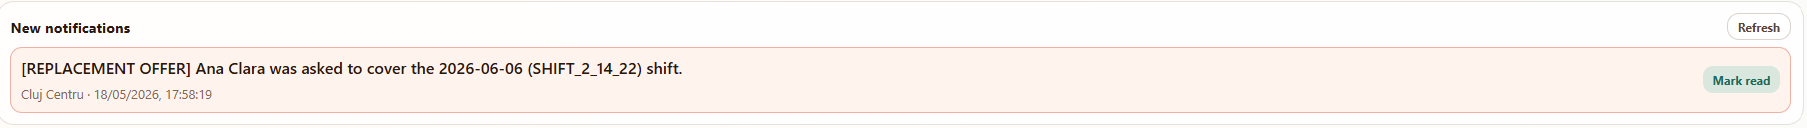
\includegraphics[width=1\linewidth]{ReplacementOffer2.png}
    \caption{Replacement offer flow - acknowledge phase 2}
    \label{fig:placeholder2}
\end{figure}

\begin{figure}[!h]
    \centering
    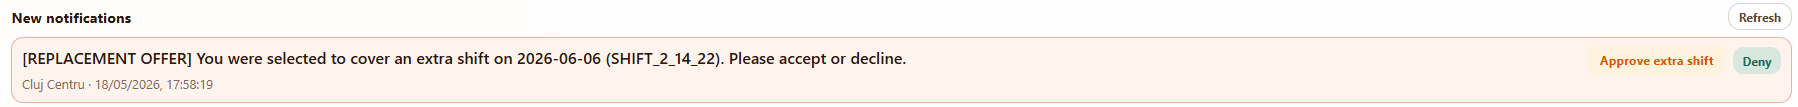
\includegraphics[width=1\linewidth]{ReplacementOffer3.png}
    \caption{Replacement offer flow - denial phase}
    \label{fig:placeholder3}
\end{figure}

\begin{figure}[!h]
    \centering
    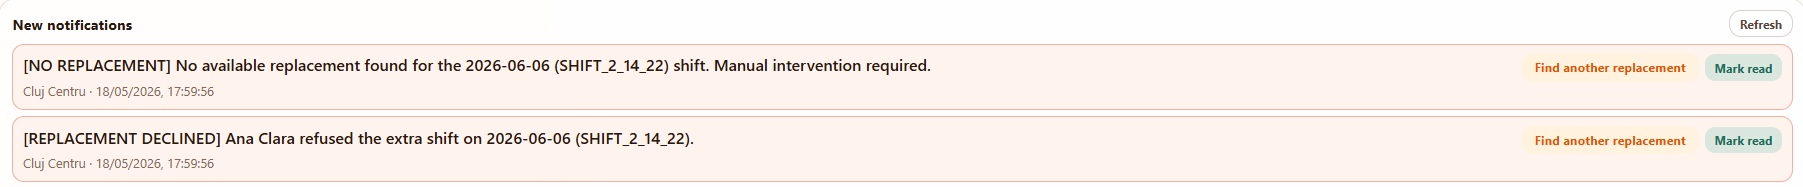
\includegraphics[width=1\linewidth]{ReplacementOffer4.png}
    \caption{Replacement offer flow - no replacement phase}
    \label{fig:placeholder4}
\end{figure}

%===========================================================
\section{Manual Operations and Schedule Adaptability}
\label{sec:manual_operations_and_schedule_adaptability}
%===========================================================

\subsection{Leave request flow}
\par The leave request system handles planned employee absences through a structured approval workflow that integrates directly with the scheduling and balance tracking subsystems.

\par Employees can submit leave requests for the second next calendar month only. This restriction is intentional: the scheduling algorithm runs a month at a time, for the next month, and confining leave requests to the upcoming month ensures that approved absences can be incorporated before the schedule is generated. Requests targeting past dates or the current month are rejected with an explicit error.

\par Before a request is accepted, the system validates several conditions:

\begin{itemize}
    \item The requesting user must be an employee (managers and administrators cannot submit leave requests through this endpoint).
    \item The requested date range must not overlap with any existing pending or approved leave request for the same employee, preventing double-booking of absence periods.
    \item The employee must have a positive remaining leave day balance; exhausted balances are reported to the employee with a suggestion to contact the manager directly.
    \item The number of calendar days requested must not exceed the remaining balance after accounting for the deductible day calculation.
\end{itemize}

\par The deductible day calculation applies a factor of 5/7 to the number of calendar days, reflecting the convention that only working days count against the leave balance. The result is rounded up to the nearest integer. For example, requesting seven calendar days deducts five leave days from the balance. This calculation is disclosed to the employee in the notification they receive after submitting the request. This measure is taken due to the special working hours that our stores use, from 10:00 to 22:00 each day of the week, leaving no free weekend days like in most of the other businesses.

\par Once the request is created, a \texttt{[LEAVE REQUEST]} notification is sent to the store manager, including the employee's name, the requested date range, the total calendar days, and the deductible count. The manager can then approve or deny the request directly from the notifications page.

\vspace{1.5em}
\begin{table}[h!]
    \centering
    \renewcommand{\arraystretch}{1.5} % Adds breathing room between rows
    \begin{tabular}{|l|p{6cm}|p{6cm}|}
        \hline
        \textbf{Action / Impact} & \textbf{Leave Approval} & \textbf{Leave Denial} \\ \hline
        \textbf{Entity Status} & Marked as \texttt{APPROVED} & Marked as \texttt{DENIED} \\ \hline
        \textbf{Data Logged} & Decision timestamp recorded & Optional textual reason stored on the entity \\ \hline
        \textbf{Leave Balance} & Deductible day count is subtracted & No change \\ \hline
        \textbf{Scheduling Engine} & Employee excluded from generation; zero shifts assigned during leave period & Standard scheduling applies \\ \hline
        \textbf{Notifications} & Confirmation sent to both the Manager (audit) and the Employee & Rejection sent to the Employee (including the reason if provided) \\ \hline
        \textbf{Follow-Up Action} & UI offers the Manager a "Regenerate month" action to fill newly vacant slots & None \\ \hline
    \end{tabular}
    \caption{Comparison of system actions based on the manager's leave request decision.}
    \label{tab:leave_decision_matrix}
\end{table}
\vspace{1.5em}

\subsection{Manual shift management}
\par Automated schedule generation covers the majority of operational cases, but real-world retail frequently requires targeted adjustments that fall outside the standard scheduling cycle. To address this, the system provides a manual shift management interface accessible to managers.

\subsubsection*{Adding a shift manually}
\par Managers can add individual shifts by selecting an employee, a date, and a shift type from the calendar interface. Before the shift is created, the backend applies the same constraint validation used by the automatic scheduler.

\begin{figure}[!h]
    \centering
    \begin{tikzpicture}[
        node distance=0.7cm,
        startbox/.style={rectangle, draw=blue!70, thick, fill=blue!5, text width=8.5cm, align=center, rounded corners=1ex, minimum height=0.8cm, font=\sffamily\bfseries},
        processbox/.style={rectangle, draw=black!70, thick, fill=gray!5, text width=8.5cm, align=left, rounded corners=1ex, minimum height=0.9cm, font=\sffamily\small},
        failbox/.style={rectangle, draw=red!70, thick, fill=red!5, text width=2.5cm, align=center, rounded corners=1ex, minimum height=0.8cm, font=\sffamily\footnotesize\bfseries},
        successbox/.style={rectangle, draw=green!70, thick, fill=green!5, text width=8.5cm, align=center, rounded corners=1ex, minimum height=0.8cm, font=\sffamily\bfseries},
        arrow/.style={thick, ->, >=stealth, draw=black!70},
        failarrow/.style={thick, ->, >=stealth, draw=red!70}
    ]

    % Nodes
    \node (start) [startbox] {Manual Shift Assignment Request};
    
    \node (step1) [processbox, below=0.8cm of start] {\textbf{1. Context Verification} \\ Verify that the targeted employee belongs strictly to the requesting manager's store.};
    
    \node (step2) [processbox, below=of step1] {\textbf{2. Eligibility Engine Execution} \\ Invoke \texttt{getEligibleEmployees} to rebuild tracker state and apply hard constraints: \\ 
    $\bullet$ Consecutive-day \& Weekly-hour limits \\ 
    $\bullet$ 12-hour back-to-back prohibition \\ 
    $\bullet$ Approved leave validation \\ 
    $\bullet$ Duplicate scheduling prevention};
    
    \node (step3) [processbox, below=of step2] {\textbf{3. Candidate Inclusion Check} \\ Verify that the specified employee exists within the newly generated eligible candidate set.};
    
    \node (step4) [processbox, below=of step3] {\textbf{4. Final Overlap Guard} \\ Perform a final validation to ensure the employee is not already assigned a shift on the target date.};
    
    \node (success) [successbox, below=0.8cm of step4] {Assignment Approved \& Persisted};

    % Fail Nodes
    \node (fail1) [failbox, right=1cm of step1] {Rejected};
    \node (fail2) [failbox, right=1cm of step2] {Rejected};
    \node (fail3) [failbox, right=1cm of step3] {Rejected};
    \node (fail4) [failbox, right=1cm of step4] {Rejected};

    % Pass Arrows
    \draw [arrow] (start) -- (step1);
    \draw [arrow] (step1) -- node[left, font=\sffamily\footnotesize] {Pass} (step2);
    \draw [arrow] (step2) -- node[left, font=\sffamily\footnotesize] {Pass} (step3);
    \draw [arrow] (step3) -- node[left, font=\sffamily\footnotesize] {Pass} (step4);
    \draw [arrow] (step4) -- node[left, font=\sffamily\footnotesize] {Pass} (success);

    % Fail Arrows
    \draw [failarrow] (step1.east) -- node[above, font=\sffamily\footnotesize] {Fail} (fail1.west);
    \draw [failarrow] (step2.east) -- node[above, font=\sffamily\footnotesize] {Fail} (fail2.west);
    \draw [failarrow] (step3.east) -- node[above, font=\sffamily\footnotesize] {Fail} (fail3.west);
    \draw [failarrow] (step4.east) -- node[above, font=\sffamily\footnotesize] {Fail} (fail4.west);

    \end{tikzpicture}
    \caption{Sequential validation and constraint pipeline for manual shift assignments.}
    \label{fig:manual_assignment_pipeline}
\end{figure}

\par If all checks pass, the shift is persisted with status \texttt{SCHEDULED} and the employee receives a \texttt{[NEW SHIFT]} notification informing them of the new assignment.

\par The frontend supports this flow by first calling a dedicated eligibility endpoint that returns the pre-filtered list of eligible employees for a given date and shift type. This allows the UI to populate the employee selector only with valid choices, providing a guided experience for the manager and eliminating the possibility of selecting an ineligible employee before the form is submitted.

\subsubsection*{Deleting a shift}
\par Managers can delete individual shifts directly from the calendar. The backend verifies that the shift belongs to the manager's store before proceeding with the deletion. Upon deletion, the affected employee receives a \texttt{[SHIFT REMOVED]} notification informing them that the assignment has been cancelled.

\par Shift deletion does not automatically trigger a replacement search intentionally, since the removal is typically an intentional managerial correction rather than an unexpected absence. If the manager needs to fill the vacated slot, they can use the manual add flow described above.

\subsection{Regeneration and data consistency during schedule updates}
\par Managers can regenerate the schedule for the next calendar month at any time. The most common scenarios are: a new employee is added to the store, a sales forecast file is updated with revised projections, or the manager simply wants to recalculate in case of a special occasion.

\par A critical correctness concern is that existing shifts may have linked absence requests, which in turn may have linked replacement offers. Deleting shifts without first removing these child records violates foreign key constraints at the database level. The regeneration logic therefore executes a cascading cleanup: it first identifies all absence request IDs linked to the shifts being removed, then deletes all replacement offers referencing those absence requests, then deletes the absence requests themselves, and finally deletes the shifts. This strict ordering ensures transactional integrity without requiring cascading deletes to be configured at the schema level, which would make the deletion behavior less visible in application code.

\par Additionally, the algorithm is specifically engineered to keep the approved leave requests in case of an emergency, therefore employees are not required to request again. This happens by keeping a \texttt{LeaveMap} function, which preserves the LeaveRequests table in the database, and freshly fetches the data for the specific month upon the time of re-generation. Instead of the scheduling algorithm constantly asking the database who is on vacation each day, it only asks the database once, builds this dictionary, and holds it in memory for the O(1) lookups.

\begin{figure}[!h]
    \centering
    
\includegraphics[width=1\linewidth]{figures/LeaveMap.png}
    \caption{buildLeaveMapFunction}
    \label{fig:placeholder_leavemap}
\end{figure}

%===========================================================
\section{System Integration and Communication}
\label{sec:system_integration_and_communication}
%===========================================================

\subsection{Notification system design}
\par All inter-role communication in QuickShift is mediated through a structured notification system. Each \texttt{Notification} entity stores a message string, the target user, the associated store, a read flag, and up to three optional foreign key references: a related absence request ID, a related leave request ID, and a related replacement offer ID.

\par These references allow the frontend to determine the action buttons to render for each notification without embedding workflow logic in the message text. The notification type is instead inferred from the message prefix (\texttt{[ABSENCE REQUEST]}, \texttt{[LEAVE REQUEST]}, \texttt{[REPLACEMENT OFFER]}, \texttt{[NO REPLACEMENT]}, and so on), which keeps the message human-readable while still being machine-parseable.

\par Notifications are marked as read in three ways: explicitly by the user clicking a read action, automatically after the user successfully completes the associated workflow action, or as a side effect of loading a new notification list after a successful operation. This multi-path read mechanism ensures that notifications do not linger after their workflow is complete, while also allowing managers to dismiss informational alerts that require no further action.

\begin{figure}[!h]
    \centering
    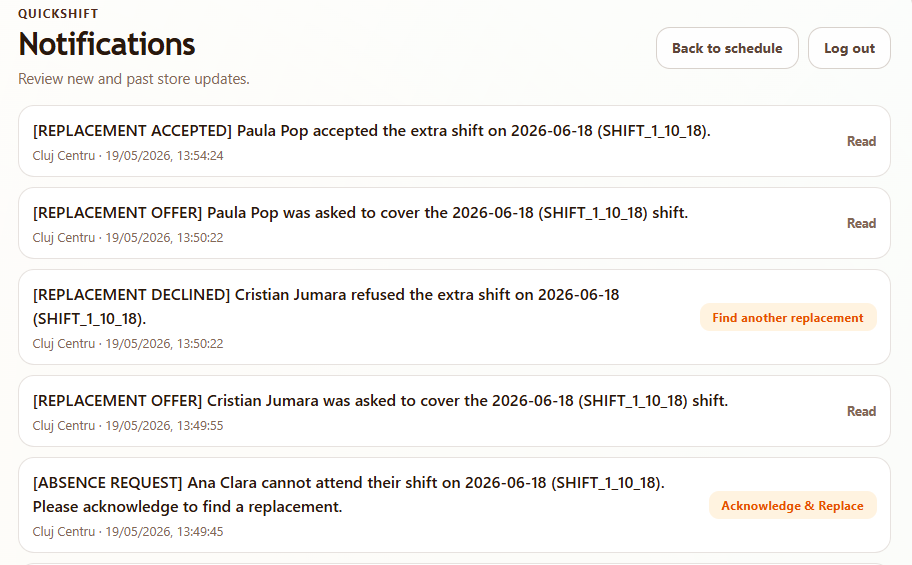
\includegraphics[width=0.7\linewidth]{NotificationPage.png}
    \caption{Notification Page design}
    \label{fig:placeholder_notif}
\end{figure}

\subsection{Complexity and practical performance considerations}
\par The main scheduling algorithm runs in $O(D \times E)$ time, where $D$ is the number of forecast days in the month and $E$ is the number of employees in scope. For typical retail stores with 30 forecast days and a team of five to fifteen employees, this is practically instantaneous.

\par The replacement algorithm has a higher constant factor because it performs a historical replay of all shifts from the beginning of the month to the absence date. The replay itself is $O(D' \times E)$ where $D'$ is the number of days elapsed in the month. However, this operation is triggered only on-demand and for a single absence event, so its cost is not on the critical path of normal scheduling operations.

\par The eligibility check for manual shift addition follows the same replay approach and has the same cost profile. Because it is user-initiated and operates on a single date, the response time is dominated by the database query rather than the computation, and is imperceptible to the user in practice.

\par By combining a fast, batch-oriented scheduling algorithm with targeted on-demand constraint checks for individual events, the implementation achieves a performance profile that is appropriate for interactive web use without requiring caching or background pre-computation.

%===========================================================
\section{Evaluation and Testing Approach}
\label{sec:evaluation_and_testing_approach}
%===========================================================

\par The system was evaluated through a multi-tiered approach, combining automated unit and integration testing with operational scenario validation. At the foundational level, a comprehensive suite of unit tests isolated and verified core business rules, while integration tests validated complex database queries and component interactions. Building upon this automated foundation, functional testing focused on verifying that the scheduler respects hard constraints across a range of forecast inputs: teams at or below the consecutive-day limit, teams with a mix of contract types, months containing approved leave, and months where sales forecasts cross both thresholds. In all tested scenarios, the generated schedule respected every hard constraint.

\par The replacement workflow was evaluated by simulating absence reports on various shift types and team compositions, including cases where the employee pool was small enough that some offers would be declined and the chain would need to proceed through multiple candidates. The auto-replacement logic correctly excluded previously declined employees in each retry and correctly identified the \texttt{UNRESOLVABLE} state when the pool was exhausted.

\par The leave request validation logic was rigorously tested for boundary conditions via integration tests targeting the database layer. These tests verified requests targeting the first and last days of the next month, requests that exactly exhaust the remaining balance, requests from employees with zero remaining balance, and precisely evaluated custom queries designed to detect all partial and total date overlaps with existing approved leave. All boundary cases produced the expected outcome.

\par To guarantee runtime auditability and facilitate real-time monitoring of complex business heuristics, a comprehensive application logging architecture was integrated using the SLF4J facade backed by the Logback framework. The system now contains over 50 strategic logging statements distributed across controllers, services, and database seeders. These logging calls are separated by severity levels to optimize performance and readability: the \texttt{INFO} level records key operational milestones (such as schedule generation runs, absence acknowledgments, and leave approval transitions), the \texttt{WARN} level captures validation failures and constraint breaches (such as role rejections or shift overlaps), and the \texttt{DEBUG} level monitors high-frequency polling events to prevent console noise. To ensure optimal execution efficiency, all log messages use SLF4J parameterized syntax (e.g., \texttt{log.info("...", arg)}), avoiding runtime string concatenation overhead unless the specific log level is active. This robust logging network provides developers and system administrators with absolute visibility into the execution flow of the CSP scheduler and the state machine transitions of the absence replacement engine.

\par User-facing evaluation focused on the click count and clarity of feedback for the most frequent workflows: generating a schedule, acknowledging an absence, approving a leave request, and adding a manual shift. Each of these workflows was designed to complete in three or fewer interactions from the point of recognizing the need for the action.
\chapter{Security and Data Protection}
\label{chap:ch5}

\par Security was treated as a primary design constraint throughout the development of QuickShift, not as a feature to be retrofitted after the core functionality was complete. The application implements stateless authentication, strict role-based access control, per-store data isolation, and a secure account lifecycle that covers both self-service password management and administrator-led provisioning of privileged accounts. This chapter describes each of these mechanisms in detail, explaining both the technical implementation and the threat model each control addresses.

%-----------------------------------------------------------
\section{Authentication Architecture and JWT-Based Sessions}
%-----------------------------------------------------------
\par The backend uses JSON Web Tokens (JWTs) as the sole session mechanism. When a user authenticates via the \texttt{/api/auth/login} endpoint, the server validates the provided credentials against the stored hashed password and, if successful, generates a signed JWT containing the user's identifier (as the subject, represented by the user's email address). The token is returned to the client and must be included as a Bearer token in the \texttt{Authorization} header of every subsequent request. \cite{JWTDepth}

\par Token validation is performed by a \texttt{JwtAuthenticationFilter} that intercepts requests before they reach any controller. The filter extracts the token from the \texttt{Authorization} header, verifies its signature and expiration using the server-side secret key, and then loads the user details via the configured \texttt{UserDetailsService}. This step queries the database on each authenticated request to obtain the current user and authorities. The filter populates Spring Security's \texttt{SecurityContext} with a \texttt{UsernamePasswordAuthenticationToken}, so controllers and service methods can access the current user through the standard \texttt{Authentication} object.

\par The stateless model eliminates server-side session storage and the associated concurrency and scalability concerns. It also mitigates the possibility of session fixation attacks, since there is no server-maintained session that an attacker could hijack by obtaining a pre-authentication identifier. The trade-off is that token revocation requires either short expiry windows or a token blacklist; the current implementation uses a fixed expiry duration configured via application properties, which is appropriate for the expected usage patterns of a store management tool.\cite{Stateless}

\par Because the token only carries the subject (user email) and not roles, authorization decisions rely on the authorities loaded from the database during the filter phase. This is much safer, because any role change or account disablement takes effect immediately, even if a previously issued token is still valid. Those authorities are then available for downstream access checks through Spring Security.

\begin{figure}[H]
    \centering
    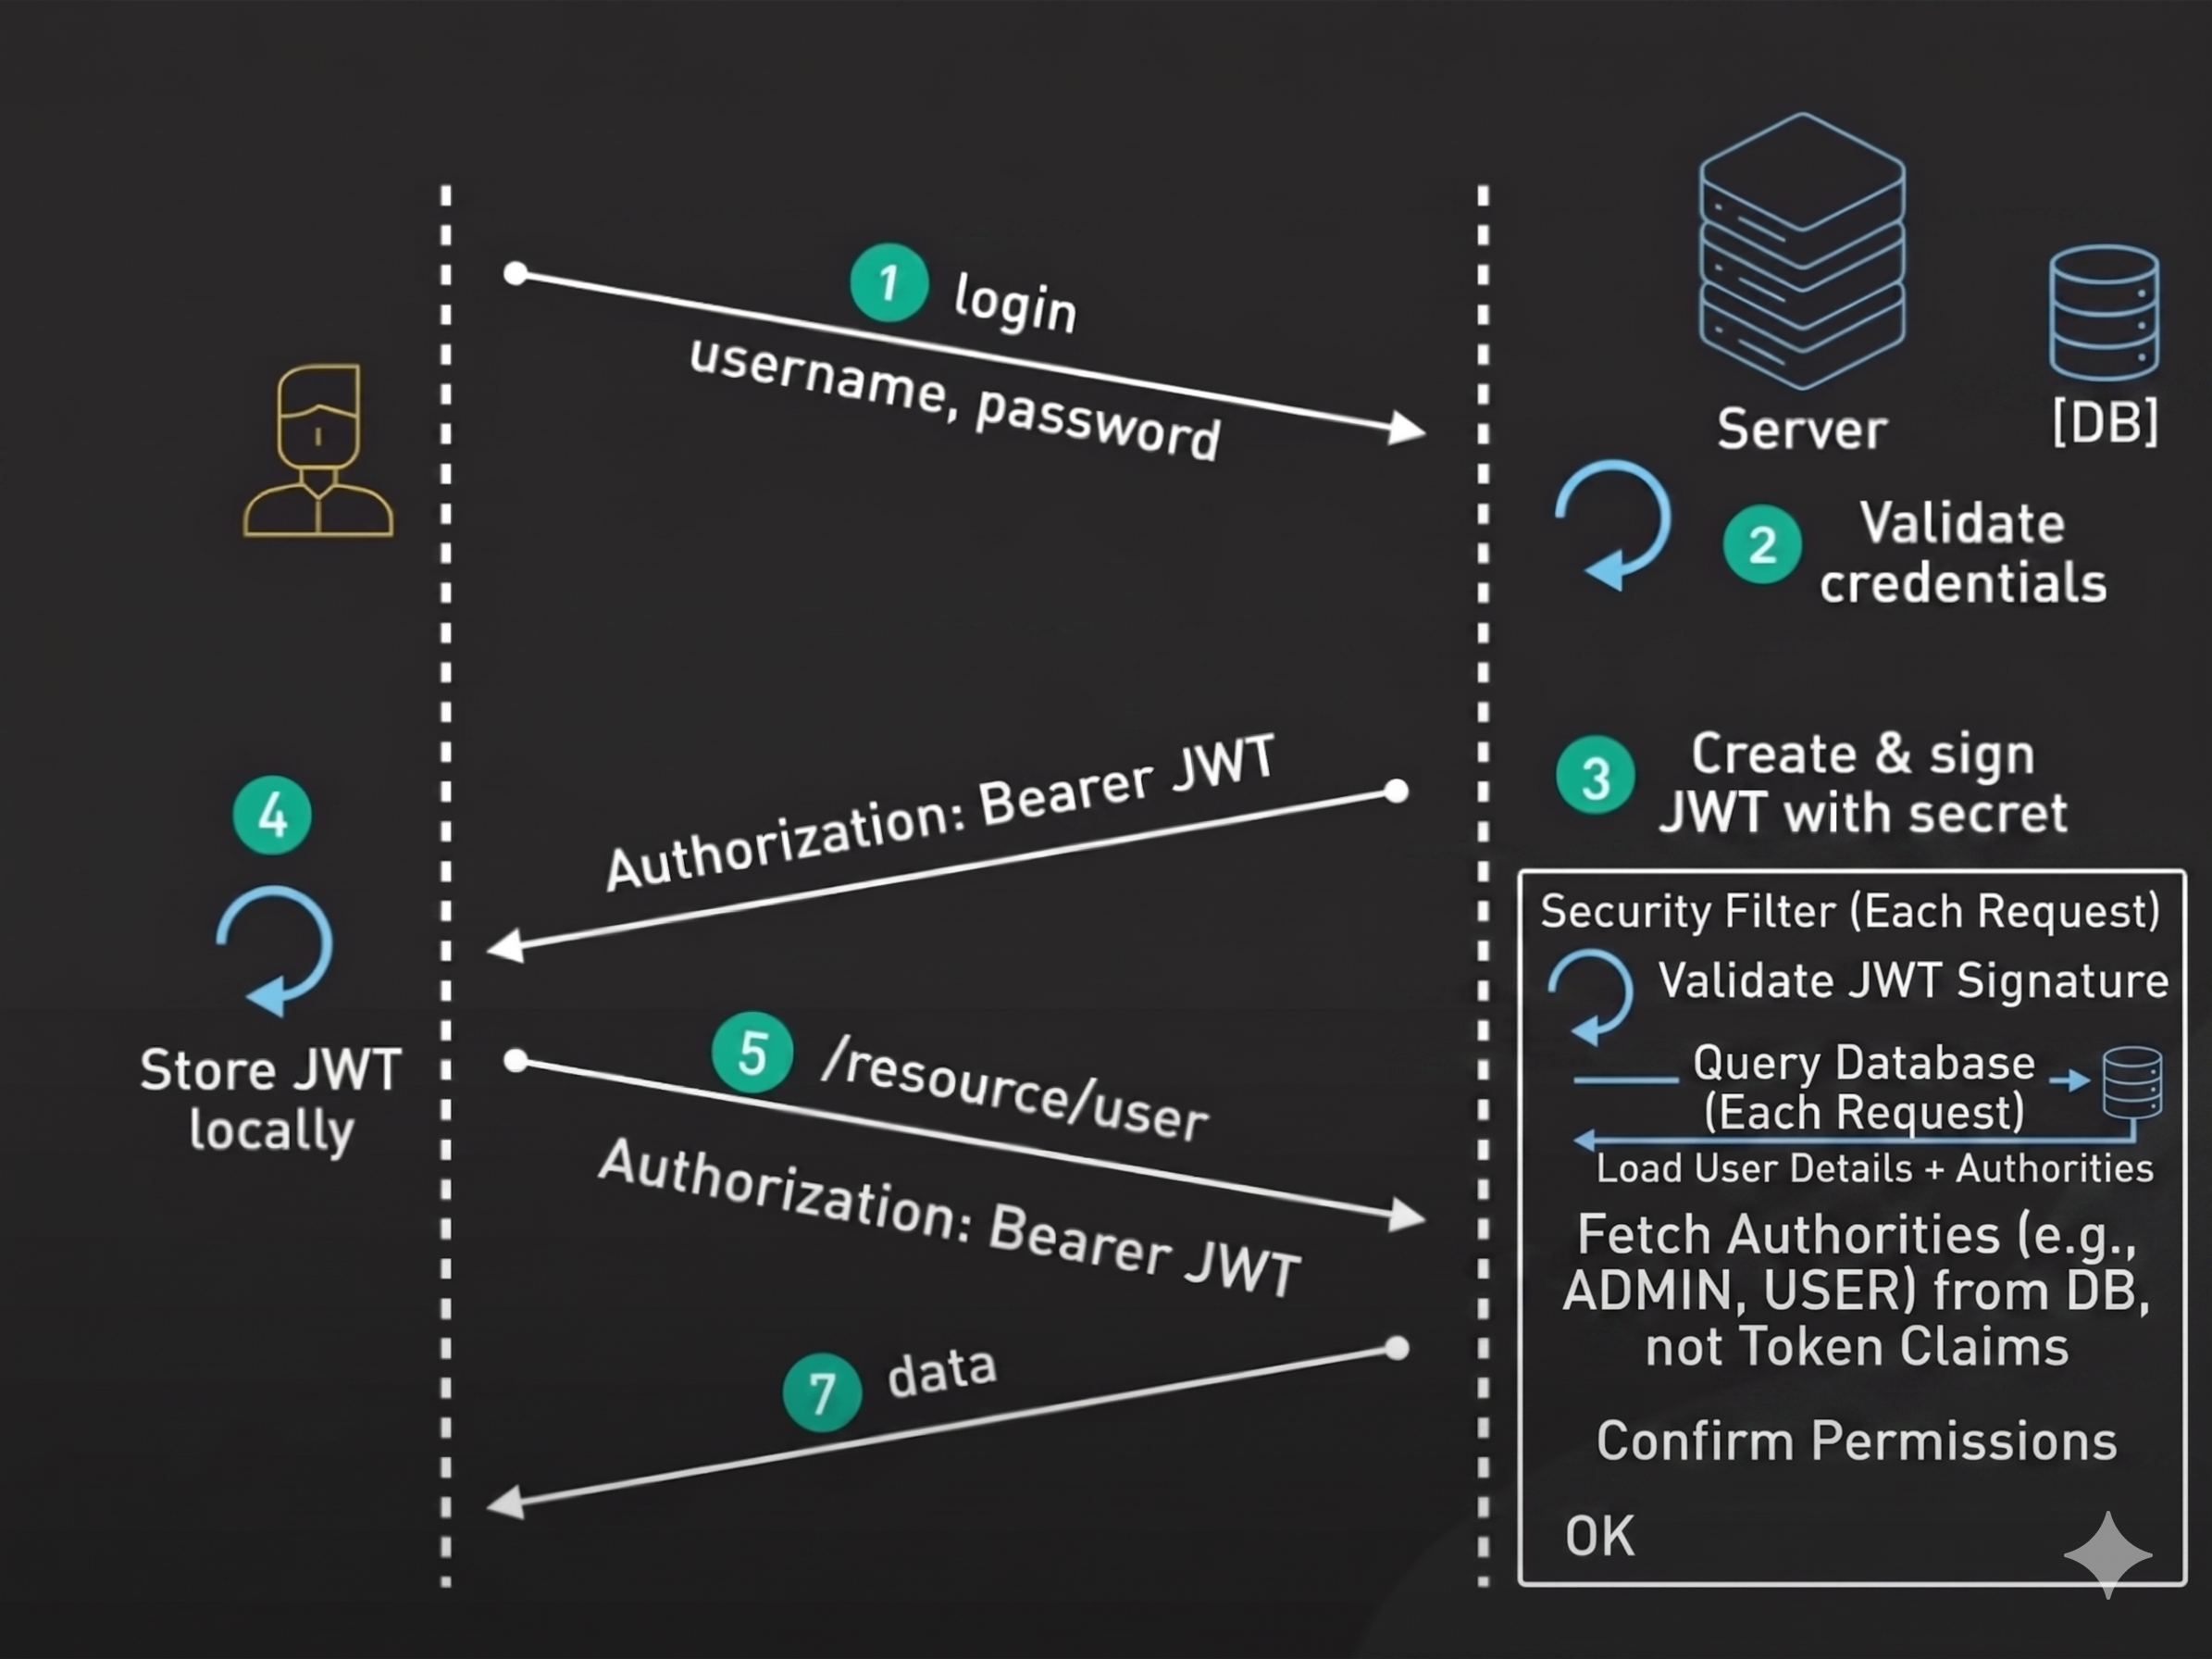
\includegraphics[width=1\linewidth]{Stateless.png}
    \caption{Stateless Authentication Visual}
    \label{fig:placeholder}
\end{figure}

%-----------------------------------------------------------
\section{Role-Based Access Control}
%-----------------------------------------------------------
\par The system defines three roles: \texttt{EMPLOYEE}, \texttt{MANAGER}, and \texttt{ADMIN}. Access control is enforced at two levels: at the HTTP layer through Spring Security's URL-based rules, and at the controller method level through explicit role checks.\cite{RBAC1}

\par URL-based rules in \texttt{SecurityConfig} restrict access to sensitive endpoint prefixes by role. For example, administrative endpoints such as store creation and manager provisioning are restricted to the \texttt{ADMIN} role, while schedule generation and absence acknowledgment are restricted to \texttt{MANAGER} and \texttt{ADMIN}. The remaining employee-facing endpoints are accessible to all authenticated users, with finer-grained ownership checks performed inside the service layer.


\par Method-level checks complement the URL rules for cases where the same endpoint serves multiple roles but must return or accept different data depending on who is calling. For example, the shift listing endpoint returns all shifts for a store when called by a manager, but only personal shifts when called by an employee. This branching logic is implemented in the controller by inspecting the role from the \texttt{Authentication} object and delegating to the appropriate service method.

\par The role separation also limits the blast radius of a compromised credential. An employee account cannot be used to access the schedule generation endpoint, acknowledge absences, or view another employee's personal data. A manager account cannot access global administrative operations such as creating new stores or provisioning other managers. This defense-in-depth approach ensures that even if an account is compromised, the attacker's capabilities are confined to the role's intended scope. \cite{RBAC2}

\begin{center}
\begin{tabular}{c}
Authentication Filter \\
$\downarrow$ \\
JWT Validation \\
$\downarrow$ \\
User Lookup \\
$\downarrow$ \\
Authority/Role Lookup \\
$\downarrow$ \\
Permission Evaluation \\
$\downarrow$ \\
Controller/Resource \\
\end{tabular}
\end{center}

%-----------------------------------------------------------
\section{Store-Scoped Data Isolation}
%-----------------------------------------------------------
\par QuickShift is designed as a multi-tenant system in which each store operates as an isolated organizational unit. Data isolation is enforced at the query level: every repository method that returns operational data (shifts, employees, leave requests, absence requests) accepts a store identifier as a parameter and filters results accordingly.

\par When a manager makes a request, their associated store identifier is extracted from their \texttt{AppUser} entity (which is loaded during the authentication filter phase) and injected into the query. This happens transparently at the service layer, so managers cannot access or modify data from stores they do not own simply by supplying a different store ID in the request body. The service method resolves the store from the authenticated user's identity rather than trusting the client-supplied value.

\par Administrators occupy a special position in this model: they are not assigned to a specific store and can therefore pass explicit store identifiers in requests. Administrative endpoints validate that the supplied store ID corresponds to an existing store before proceeding, so even administrators cannot target non-existent stores. Global operations (such as listing all employees across all stores) are available only to administrators and not to managers.

\par This isolation model prevents horizontal privilege escalation between tenants: a compromised manager account for store A cannot be used to read or modify data for store B, since the store association is enforced server-side from the authenticated identity rather than from any client-controlled parameter.

\begin{figure}[H]
\centering
\begin{tikzpicture}[
    node distance=4cm and 4cm, % Increased vertical distance to prevent overlapping
    role/.style={
        rectangle,
        rounded corners,
        draw=black,
        thick,
        minimum width=4cm,
        minimum height=1.2cm,
        align=center,
        fill=gray!10
    },
    access/.style={
        rectangle,
        draw=black,
        minimum width=5.5cm, % Slightly widened to better fit the new text
        minimum height=2.2cm,
        align=left,
        fill=blue!5
    },
    arrow/.style={
        ->,
        thick
    }
]

% Roles
\node[role] (admin) {\textbf{ADMIN}};
\node[role, below=of admin] (manager) {\textbf{MANAGER}};
\node[role, below=of manager] (employee) {\textbf{EMPLOYEE}};

% Permissions
\node[access, right=4cm of admin] (adminacc) {
\textbf{Access Scope:} \\
$\bullet$ All stores \\
$\bullet$ User provisioning \\
$\bullet$ Store management \\
$\bullet$ Shift management \\
$\bullet$ Employee management \\
$\bullet$ Full administrative operations
};

\node[access, right=2cm of manager] (manageracc) {
\textbf{Access Scope:} \\
$\bullet$ Own store only \\
$\bullet$ Employee management \\
$\bullet$ Shift generation and updates \\
$\bullet$ Manual shift management \\
$\bullet$ Absence acknowledgment and replacement \\
$\bullet$ Leave request approval/disapproval \\
};

\node[access, right=4cm of employee] (employeeacc) {
\textbf{Access Scope:} \\
$\bullet$ Own store only \\
$\bullet$ View personal schedule \\
$\bullet$ Report absences \\
$\bullet$ Request Leave \\
};

% Arrows
\draw[arrow] (admin) -- (adminacc);
\draw[arrow] (manager) -- (manageracc);
\draw[arrow] (employee) -- (employeeacc);

\end{tikzpicture}

\caption{Role-based access control hierarchy and permission scope.}
\label{fig:rbac}
\end{figure}

%-----------------------------------------------------------
\section{Secure Password Management and Recovery}
%-----------------------------------------------------------
\par To protect user credentials throughout their lifecycle, QuickShift implements a secure password storage strategy, an authenticated change workflow, and a time-limited recovery mechanism.

%-----------------------------------------------------------
\subsection{Password Storage and Authenticated Change Workflow}
%-----------------------------------------------------------
\par User passwords are stored exclusively in encoded form. The \texttt{PasswordEncoder} bean configured in the Spring Security context applies a strong hashing algorithm (BCrypt\cite{bcrypt1999} by default in the Spring Security ecosystem) before any password is persisted. The raw password is never stored, logged, or returned in any API response.

\par Authenticated users can change their own password through a dedicated endpoint that requires the caller to supply their current password. The endpoint verifies the current password against the stored hash before accepting the new one. This requirement prevents an attacker who has gained temporary access to an authenticated session (for example, through a shared or unattended device) from silently changing the account password and locking out the legitimate owner.

\par New passwords are immediately encoded and stored, replacing the previous hash. The old password becomes invalid at the moment the change is committed, so subsequent requests using a JWT that was issued before the change will still be valid until the token expires, since the token is not invalidated by a password change. 

%-----------------------------------------------------------
\subsection{Forgot-Password and Time-Limited Recovery Tokens}
%-----------------------------------------------------------
\par The password recovery flow is designed to be both secure and frictionless for legitimate users. When an employee or manager requests a password reset, the system generates a cryptographically random token, associates it with the requesting account, and stores it in the \texttt{PasswordResetToken} table with a 15-minute expiry and a \texttt{used} boolean flag initialized to \texttt{false}. A reset link embedding the token is then sent to the user's registered email address.

\par When the user follows the link and submits a new password, the backend validates the token in three steps as summarized in Table~\ref{tab:token_validation}.

\begin{table}[H]
\centering
\begin{tabular}{|p{3.5cm}|p{6.5cm}|p{4.5cm}|}
\hline
\textbf{Validation Check} & \textbf{Mechanism/Database Field} & \textbf{Failure Consequence} \\ \hline
Token Existence & Query by token string & Immediate rejection (Unknown Token) \\ \hline
Expiration Check & Compare \texttt{expiresAt} with current time & Rejection (Expired Token) \\ \hline
Usage Status & Verify \texttt{used} boolean flag is \texttt{false} & Rejection (Already Used Token) \\ \hline
\end{tabular}
\caption{Step-by-step token validation checks for password recovery.}
\label{tab:token_validation}
\end{table}

\par If all three checks pass, the new password is encoded and stored, and the token's \texttt{used} flag is set to \texttt{true}. This invalidates the token for any future use, preventing replay attacks in which an attacker who intercepts a reset link could apply it a second time after the legitimate user has already completed the reset.

\par The 15-minute expiry window is short enough to limit the risk of interception but long enough to accommodate realistic email delivery delays and user response times.

%-----------------------------------------------------------
\section{Input Validation and Structured Error Handling}
%-----------------------------------------------------------
\par All publicly exposed endpoints apply input validation before invoking service logic. Mandatory fields are checked for presence, date ranges are validated for logical consistency (end date must not precede start date), and string values that must match an enumerated set are validated against that set. Malformed or logically inconsistent requests are rejected with HTTP 400 and a descriptive error message before any database operation is attempted.

\par Error messages are kept concrete enough to be actionable for legitimate users but deliberately do not expose internal implementation details such as stack traces, database column names, or query structures. For 401 and 403 responses, the messages are intentionally generic to avoid leaking information about which accounts or resources exist.

\par In the frontend, error responses from the backend are displayed inline within the relevant form or notification component rather than through modal dialogs or global alert banners. This keeps the error context local to the action that caused it and reduces user confusion. Errors are cleared when the user modifies the input or retakes the relevant action.

%-----------------------------------------------------------
\section{Transactional Safeguards for Multi-Step Operations}
%-----------------------------------------------------------
\par Several operational flows in QuickShift involve multiple related writes that must either all succeed or all fail together. Table~\ref{tab:transactional_safeguards} details these critical flows and the potential inconsistencies that would arise from partial failures.

\begin{table}[H]
\centering
\begin{tabular}{|p{4.5cm}|p{9.5cm}|}
\hline
\textbf{Operational Flow} & \textbf{Atomic Actions and Inconsistency Risks} \\ \hline
\textbf{Leave Approval} & Deducting leave days, updating request status, and marking shifts as absent. A partial failure would leave the leave balance inconsistent. \\ \hline
\textbf{Replacement Offer} & Creating the replacement shift, updating the absence request status, and updating the offer status. A failure would leave the slot marked unfilled. \\ \hline
\textbf{Schedule Regeneration} & Deleting existing shifts, absence requests, and replacement offers, followed by generating the new schedule. A failure would leave the store with no schedule. \\ \hline
\end{tabular}
\caption{Critical transactional bounds and inconsistency risks.}
\label{tab:transactional_safeguards}
\end{table}

\par All service methods that perform multi-step writes use the \texttt{@Transactional} annotation  \cite{spring_transactional}, delegating the consistency guarantee to the Spring transaction manager and the underlying database. If any step in the method throws an exception, the entire transaction is rolled back and the database is restored to its state before the method was invoked.

%-----------------------------------------------------------
\section{Email Infrastructure and Security Notifications}
%-----------------------------------------------------------
\par QuickShift integrates email delivery to support both manager onboarding workflows and automated security notifications for user password resets.

%-----------------------------------------------------------
\subsection{Manager Onboarding and Account Provisioning}
%-----------------------------------------------------------
\par Manager accounts are created exclusively by administrators through a dedicated provisioning endpoint. This design prevents self-registration of privileged accounts and maintains a controlled, auditable onboarding process for store managers.

\par When an administrator provisions a new manager, the system follows the sequence of steps detailed in Table~\ref{tab:manager_provisioning}.

\begin{table}[H]
\centering
\begin{tabular}{|c|l|p{9.5cm}|}
\hline
\textbf{Step} & \textbf{Action} & \textbf{Implementation Details} \\ \hline
1 & Password Generation & Generates a secure, cryptographically random temporary password. \\ \hline
2 & User Record Creation & Creates the \texttt{AppUser} record with the \texttt{MANAGER} role and the encoded temporary password. \\ \hline
3 & Email Dispatch & Sends an onboarding email to the manager containing the credentials and setup instructions. \\ \hline
\end{tabular}
\caption{Manager account provisioning workflow sequence.}
\label{tab:manager_provisioning}
\end{table}

\par The administrator also assigns the new manager to a specific store at provisioning time, using a dropdown populated from the list of stores that do not yet have an assigned manager. This prevents creating orphaned manager accounts and keeps the store-manager relationship consistent from the moment of account creation.

%-----------------------------------------------------------
\subsection{Email Delivery for Security-Critical Communications}
%-----------------------------------------------------------
\par The application integrates with an SMTP server \cite{smtp_rfc5321} via Spring's \texttt{JavaMailSender} to deliver security-critical emails. The two primary categories of dispatched emails are summarized in Table~\ref{tab:email_categories}.

\begin{table}[H]
\centering
\begin{tabular}{|p{4.5cm}|p{9.5cm}|}
\hline
\textbf{Email Category} & \textbf{Contents and Security Scope} \\ \hline
\textbf{Password Reset Links} & Contains the reset URL with the embedded token, instructions, and a notice that the link expires in 15 minutes to prompt quick action. \\ \hline
\textbf{Manager Onboarding} & Contains the temporary password and instructions to log in and change it immediately before performing any operations. \\ \hline
\end{tabular}
\caption{Categories of security-critical email communications.}
\label{tab:email_categories}
\end{table}

\par Email delivery failures are not silently swallowed. If the mail server is unreachable or the message cannot be sent, the exception propagates to the controller, which returns an appropriate error to the calling client. This ensures that administrators are aware of delivery failures rather than believing a provisioning action succeeded when the manager never received their credentials.

%-----------------------------------------------------------
\section{Summary of the Security Architecture}
%-----------------------------------------------------------
\par The QuickShift security model is built on four independent layers that collectively provide defense in depth, as outlined in Table~\ref{tab:security_layers}.

\begin{table}[H]
\centering
\begin{tabular}{|l|p{10.5cm}|}
\hline
\textbf{Security Layer} & \textbf{Key Mechanism and Security Value} \\ \hline
\textbf{Authentication} & Stateless JWT-based sessions prevent session-related attacks and scale horizontally. \\ \hline
\textbf{Authorization} & Role-based access control at URL/method level and ownership checks in service logic. \\ \hline
\textbf{Data Isolation} & Store-scoped queries enforced server-side prevent horizontal cross-tenant access. \\ \hline
\textbf{Account Lifecycle} & BCrypt hashing, time-limited recovery tokens, and transactional email dispatch. \\ \hline
\end{tabular}
\caption{Defense-in-depth security layers in QuickShift.}
\label{tab:security_layers}
\end{table}

\par This layered design means that a weakness in one layer does not immediately compromise the entire system. An attacker who obtains a valid JWT is still constrained by role and store scope; one who gains access to the database sees only hashed passwords; one who intercepts a reset email has at most 15 minutes to use the token and cannot reuse it after the legitimate user resets their password.
\chapter{Frontend Implementation and Design}
\label{chap:ch6}

\par The QuickShift frontend was built as an application using React 18 and TypeScript, with Vanilla CSS for styling. The guiding design principles were operational clarity and low friction: the interface should allow a non-technical store manager to generate schedules,  review absences, and manage staff without requiring training or documentation. At the same time, the interface must expose the full complexity of the underlying workflows — replacement chains, leave approval with balance tracking, manual shift corrections — through well-structured, action-oriented components.

%-----------------------------------------------------------
\section{Project Structure}
%-----------------------------------------------------------
\par React was chosen for its component model, which maps naturally onto the page-and-panel structure of the application. TypeScript adds static typing that catches API contract mismatches at development time, which is particularly valuable when the backend response shapes evolve as new features are added. Vite is used as the build tool, providing fast hot-module replacement during development and a compact production bundle.

\par API communication is handled through the Axios library \cite{axios}, with a centralized instance configured with the base URL from an environment variable. All authenticated requests attach the JWT stored in \texttt{localStorage} via a request interceptor, so individual service functions do not need to manage the Authorization header explicitly.  Unauthorized (401) responses are handled in the authentication layer when fetching the current user and triggering the logout flow to prevent stale credentials from persisting in the UI.

\par Authentication state is managed through a custom \texttt{useAuth} hook backed by React context. The hook exposes the current user, authentication flags, and helpers to store or clear the JWT. Login flows call the API and then store the received token via the context helper, while logout clears storage and auth state; routing logic then redirects unauthenticated users to the public pages. Components consume the hook to conditionally render content based on the user’s role and authentication status.

%-----------------------------------------------------------
\subsection{Routing and Route Protection}
%-----------------------------------------------------------
\par Client-side routing is handled by React Router v6. The route configuration is centralized in the main application component, with a \texttt{ProtectedRoute} wrapper component that checks the current authentication state before rendering the target page. Unauthenticated users attempting to access protected routes are redirected to the login page; authenticated users attempting to access the login or registration pages are redirected to the schedule page.

\par Role-based routing is layered on top of authentication protection. Certain pages such as the store management screen are accessible only to administrators; the schedule and notifications pages are accessible to both managers and employees, but render different content and controls depending on the role. This approach keeps the routing table simple while still enforcing role-appropriate access at the page level.

%-----------------------------------------------------------
\section{Calendar-Centric Scheduling Interface}
%-----------------------------------------------------------
\par The calendar page is the operational hub of the application. It renders a monthly grid in which each cell corresponds to one day, and each cell may contain one or more shift cards representing scheduled employees. Shift cards display the employee's full name, the shift type, and a color-coded status indicator that distinguishes between \texttt{SCHEDULED}, \texttt{ABSENT}, and \texttt{REPLACEMENT} shifts at a glance.

\par The calendar supports two navigation dimensions: the user can move forward or backward by month using arrow controls, and can also switch between stores if they have administrator privileges. The underlying API calls are parameterized by year, month, and optionally store ID, so the calendar always shows exactly the data relevant to the selected view.

\par Schedule generation is triggered from a button in the calendar header.Upon submission by the manager of the respective store, the frontend calls the generation endpoint and re-fetches the shift list on success, so the calendar updates immediately without a full page reload.

\begin{figure}[H]
    \centering
    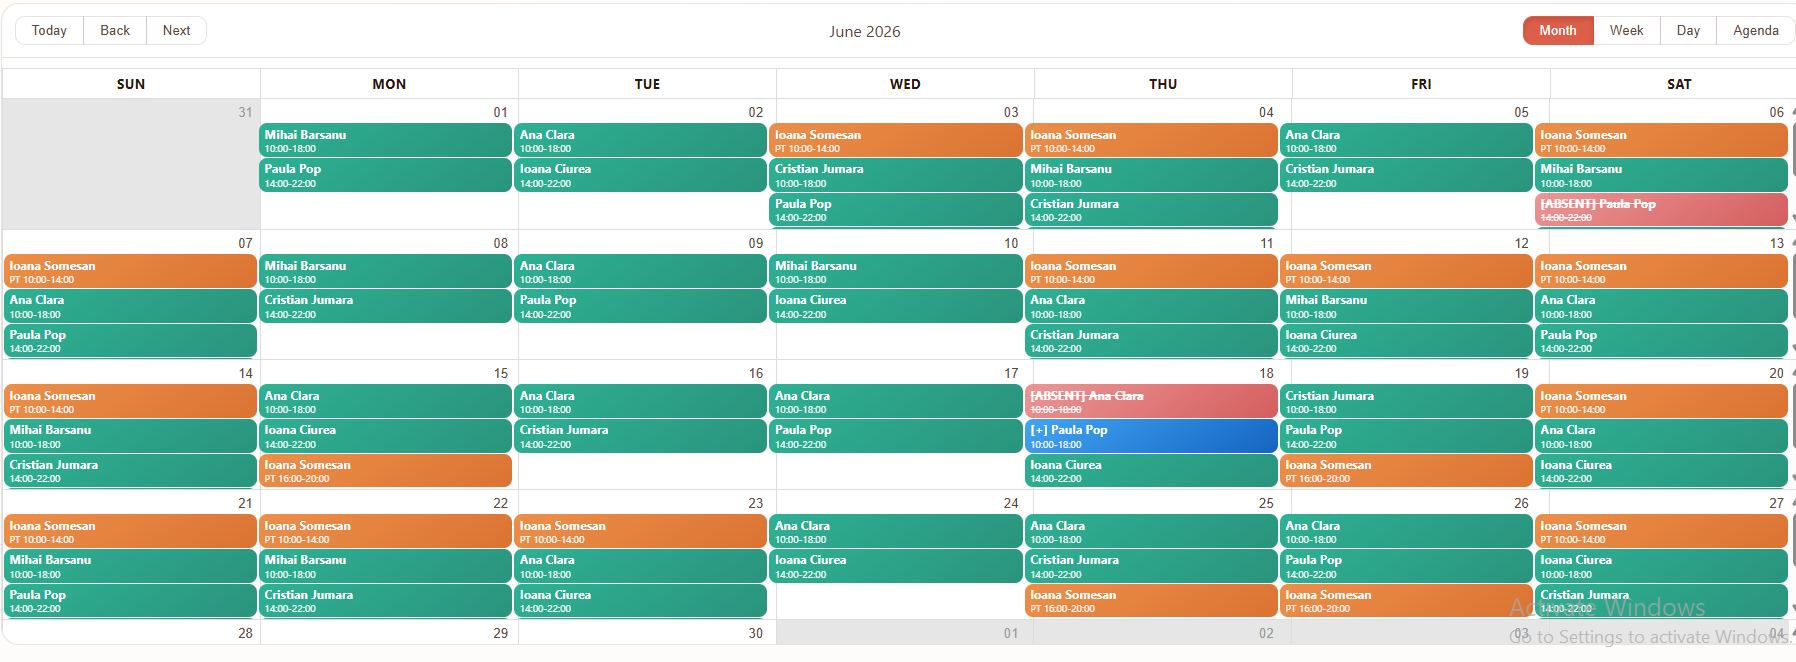
\includegraphics[width=1\linewidth]{Schedule.png}
    \caption{Main Schedule viewpoint}
    \label{fig:placeholder}
\end{figure}

\subsubsection*{Manual shift addition}

\par Managers can add individual shifts by clicking on the \texttt{Manage Shifts} button and selecting a date for the shift. The form first fetches the list of eligible employees for the selected date and shift type from the backend, populating the employee selector with only valid choices. This server-driven eligibility check ensures that the constraint logic described in Chapter 4 is enforced at the point of selection rather than only at submission time, which reduces the likelihood of a rejected submission and provides clearer guidance to the manager.

\par After selecting an employee and confirming, the frontend calls the shift creation endpoint and re-renders the relevant calendar cell on success. An error returned by the backend (for example, if the employee becomes ineligible between the time the form was opened and the time of submission) is displayed inline in the form panel.

\subsubsection*{Shift deletion}

\par Managers can delete a shift by clicking on the remove action from the same \texttt{Manage Shifts} menu. There, all the scheduled shifts for the selected date, alongside the addition option, can be viewed. The delete endpoint is called and the card is removed from the calendar grid on success. A confirmation step is deliberately omitted to keep the interaction smooth (if the manager manually updated that shift, it is necessary to respect it); instead, the employee receives an automatic \texttt{[SHIFT REMOVED]} notification via the system, which serves as a record of the change.

\begin{figure}[H]
    \centering
    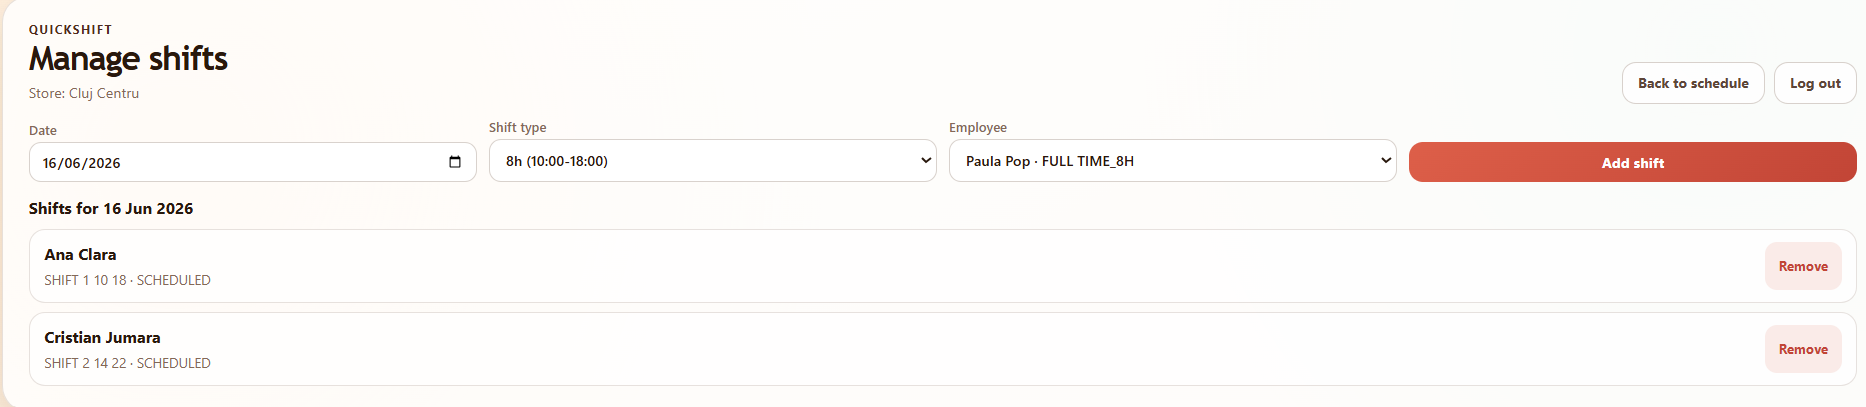
\includegraphics[width=0.5\linewidth]{Manual Shift.png}
    \caption{Manual Shift manipulations for managers overview}
    \label{fig:placeholder}
\end{figure}

%-----------------------------------------------------------
\section{My Shifts Page and Employee Self-Service}
%-----------------------------------------------------------
\par Employees interact with the system primarily through the \emph{Manage my shifts} page, which presents their personal shift schedule in a combined calendar and list view. The page shows all shifts assigned to the logged-in employee across the current and upcoming months, with the same status color coding used in the manager calendar.

\par From this page, employees can report absence for any future shift in a \texttt{SCHEDULED} or \texttt{REPLACEMENT} status. The report form asks for an optional reason, which is stored on the absence request and visible to the manager. Submitting the report creates the absence request in the backend and sends the manager notification described in Chapter 4; the shift's status does not change immediately, since the system waits for manager acknowledgment before marking it as \texttt{ABSENT}.

\par Employees can also submit leave requests from this page. A date range picker scoped to the next calendar month allows them to select the desired period, and the form displays their current remaining leave balance alongside the estimated deductible days for the selected range (calculated from the 5/7 calendar-to-working-day ratio). This real-time estimate helps employees make informed decisions before submitting, reducing the frequency of requests that exceed the available balance.

\begin{figure}[H]
    \centering
    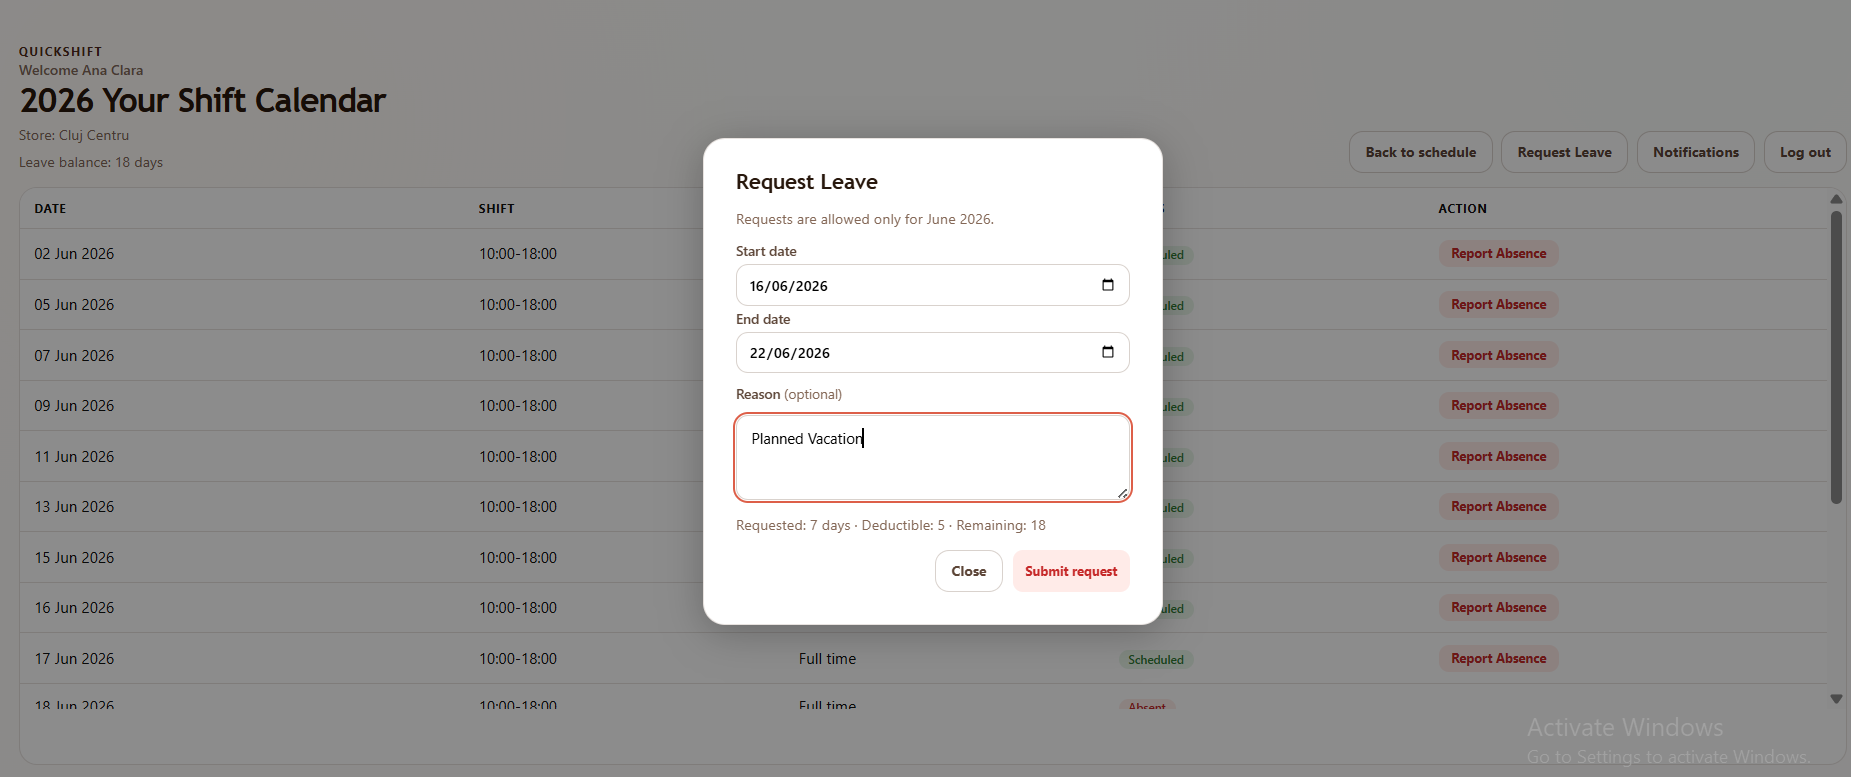
\includegraphics[width=1\linewidth]{LeaveRequest.png}
    \caption{Leave request option on the manage shifts page}
    \label{fig:placeholder}
\end{figure}

%-----------------------------------------------------------
\section{Notifications Page and Workflow Actions}
%-----------------------------------------------------------
\par The notifications page is the primary coordination surface between managers and employees. It renders a chronological list of all unread notifications for the current user on the main dashboard, with read notifications visible but visually de-emphasized on the designated notifications page. Each notification card displays the message text, the store name, and the creation timestamp.

\par The key design challenge of the notifications page is that different notification types require fundamentally different action controls, and the state of those controls must be maintained as the user interacts with them without causing the entire list to re-fetch on every action. This is solved by maintaining per-notification action state in three separate state maps within the page component: one for acknowledgment actions (absence requests), one for leave decisions, and one for replacement offer actions. Each map is keyed by notification ID, so updates to one notification do not disturb the display state of others.

\subsubsection*{Absence acknowledgment}

\par Notifications prefixed with \texttt{[ABSENCE REQUEST]} render an \emph{Acknowledge \& Replace} button. Clicking it calls the acknowledgment endpoint and updates the notification's local state to show a result message: either a success message naming the replacement employee, or a warning if no replacement was found. In the success case, the shift proposal is sent through a notification to that employee, and if they accept, a follow-up notification is sent to the manager with the person that accepted the shift.

\subsubsection*{Leave request decisions}

\par Notifications prefixed with \texttt{[LEAVE REQUEST]} render two buttons: \emph{Approve leave} and \emph{Deny}. The deny flow opens an inline panel in which the manager can enter an optional reason before confirming. In the approved state, the notification transitions to a success message and the employee also receives a confirmation of the leave request being approved. The amount of leave days remaining in the employee's balance is deducted immediately, and upon generation of the month in which the leave was requested, the employee will not be considered for any shifts in the requested period.

\subsubsection*{Replacement offer acceptance and denial}

\par Notifications prefixed with \texttt{[REPLACEMENT OFFER]} are received by employees and render \emph{Approve extra shift} and \emph{Deny} buttons. Clicking either button calls the corresponding endpoint and marks the notification as read. The system then handles the downstream consequences (creating the replacement shift on acceptance, or triggering the next automated search on denial) server-side, and the manager receives a follow-up notification reflecting the outcome.

\subsubsection*{No replacement alerts}

\par Notifications prefixed with \texttt{[NO REPLACEMENT]} are received by managers when no eligible replacement could be found for an absent shift. These notifications render a \emph{Find another replacement} button, which triggers a new automated search from the current state of the employee pool (potentially with different constraint states compared to when the original search ran). They also render a \emph{Mark as read} button so that managers can dismiss the alert after arranging a manual resolution outside the system. This dismissal path is essential for the system to remain usable when all automated options have been exhausted.

%-----------------------------------------------------------
\section{Authentication Pages and Account Recovery}
%-----------------------------------------------------------
\par The login page presents a standard email and password form with inline error feedback for authentication failures. Successful login stores the JWT and decoded user payload in \texttt{localStorage} and redirects the user to the schedule page.

\par The registration page is available to employees who self-onboard. It collects full name, email, password, contract type, shift preference, and optionally a store selection. A password confirmation field with client-side match validation reduces the likelihood of registration failures caused by typing errors. On successful registration, the user is automatically logged in and redirected to their personal shift page.

\par The forgot-password page accepts an email address and triggers the backend reset flow. The form does not indicate whether the supplied email corresponds to an existing account, preventing account enumeration attacks. After submission, the user is shown a generic confirmation message instructing them to check their email. The reset page, linked from the email, accepts the new password and its confirmation, validates both client-side for match and minimum length, and submits to the backend token validation and update endpoint.

\par The change-password page for authenticated users requires the current password, the new password, and a confirmation. Since users are already authenticated for this functionality, it does not require any restrictive attention, like the forgot password does.

%-----------------------------------------------------------
\section{Role-Specific Navigation and UI Adaptation}
%-----------------------------------------------------------
\par Navigation is rendered conditionally based on the current user's role. The navigation bar items, action buttons, and page sections visible to each role are as follows:

\begin{itemize}
    \item \textbf{Employees} see their personal shift calendar, the leave request form, the absence reporting controls, and the notifications page for replacement offer decisions.
    \item \textbf{Managers} see the store schedule calendar with generation, manual add, and delete controls; the notifications page with absence acknowledgment and leave decision controls; and the employee list for their store.
    \item \textbf{Administrators} see all of the above(except manual shift manipulation) plus the store management page, the manager provisioning form, and a global employee view across any chosen store.
\end{itemize}

\par Role-specific UI is handled within the components themselves: they read the user role from \texttt{useAuth} and conditionally render controls (e.g., manager-only actions) as needed, while routing primarily gates access based on authentication status rather than role-based route splits.\cite{fireactUseAuth}

%-----------------------------------------------------------
\subsection{Store Management and Administrator Interface}
%-----------------------------------------------------------
\par The store management page is accessible only to administrators. It provides a tabbed interface covering three areas: store creation, employee listing with store assignment, and manager provisioning.

\par Store creation requires a store name, a location identifier and a busy day threshold - which can then be updated by the managers depending on the stores' sales. After creation, the store appears immediately in the store selector used throughout the application. The administrator can then assign a manager to the store through the provisioning form, which requires an email address and the target store. The provisioning action creates the manager account, sends the onboarding email, and links the account to the selected store in a single operation.

\par The employee listing shows all registered employees grouped by store, with their contract type, shift preference, and current leave day balance visible.

\begin{figure}[H]
    \centering
    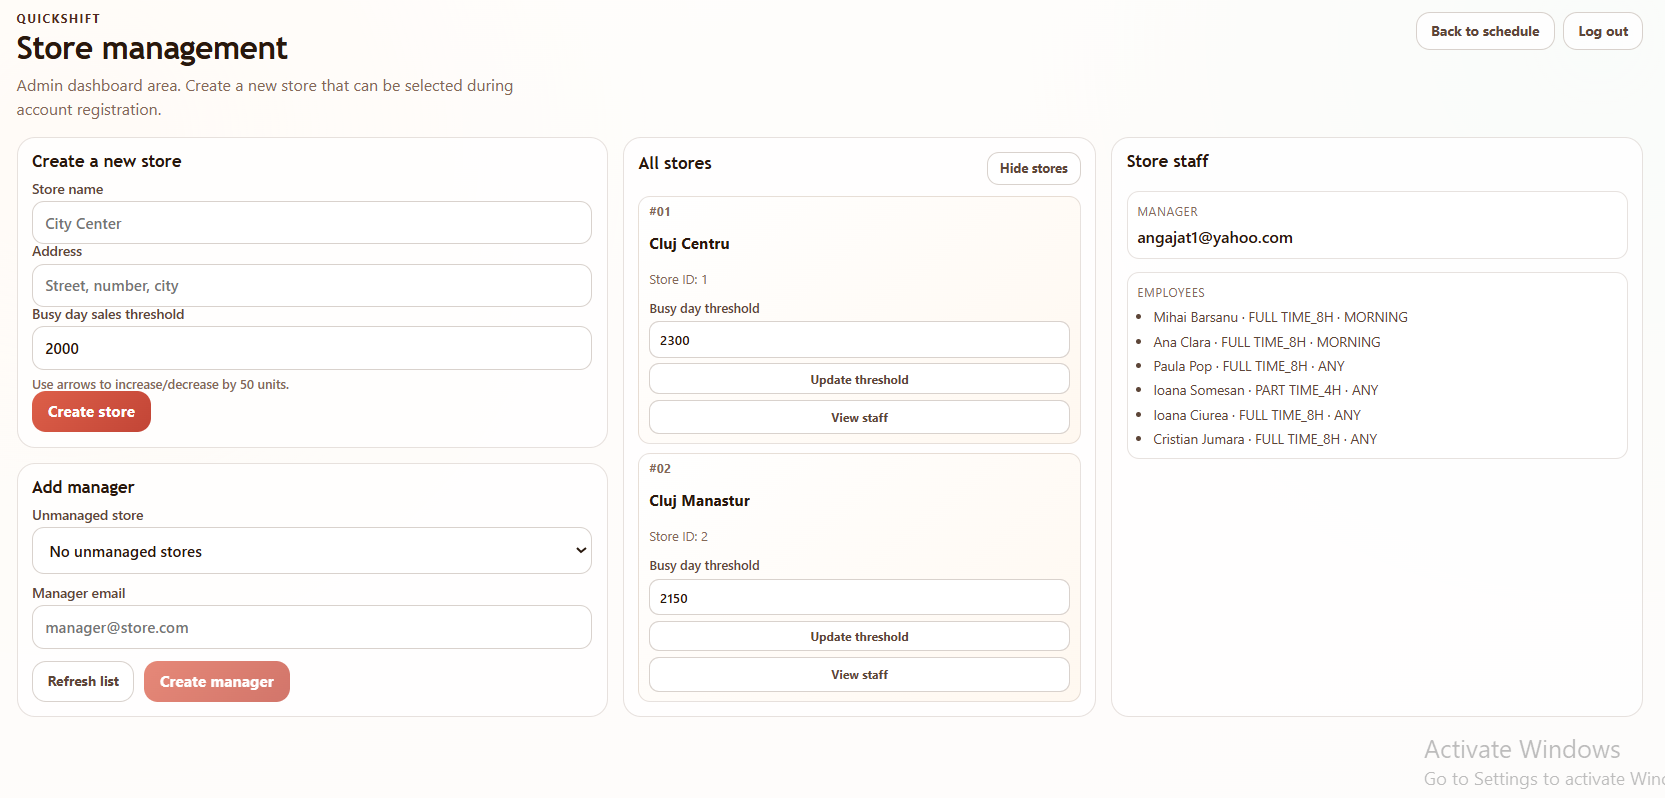
\includegraphics[width=0.7\linewidth]{ManageStores.png}
    \caption{Manage stores page overview}
    \label{fig:placeholder}
\end{figure}

%-----------------------------------------------------------
\section{Client-Side State Management Strategy}
%-----------------------------------------------------------
\par The application does not use a global state management library such as Redux. Instead, state is organized at the page level using React's built-in \texttt{useState} and \texttt{useEffect} hooks. Authentication state is the only globally shared state, distributed through a context provider.\cite{reactUseEffect}, \cite{reactUseState}

\par This choice reflects the scale of the application: the data flows are straightforward, and each page typically fetches the data it needs directly. The overhead of a global store would exceed the complexity it resolves. The trade‑off is that some data is re‑fetched more often than strictly necessary (for example, the notification list after each action), but this keeps the UI consistent with the server state and is acceptable for the expected usage volume.
\par Local action state (pending flags, error messages, inline results) is tracked in per-notification state maps as described in the notifications section, allowing fine-grained loading and error feedback without blinking the entire list on each interaction.

%-----------------------------------------------------------
\section{Styling Philosophy and Visual Design}
%-----------------------------------------------------------
\par The styling is implemented entirely in Vanilla CSS \cite{cssVanillaLayout} using custom properties (CSS variables) for the color palette and spacing scale. This allows the visual design to be adjusted globally by modifying a small set of root variables, without hunting for hardcoded values scattered across stylesheets.

\par The color system distinguishes between states through consistent cues: green for success and approved statuses, amber for warnings and pending states, red for errors and absent statuses, and a neutral dark palette for the base layout. Status badges on shift cards use these colors directly, so a manager scanning the calendar can identify problematic days at a glance without reading the text of each card.

\par Typography uses the Inter font family loaded from Google Fonts. Inter was chosen for its high legibility at small sizes and its wide character coverage, which is important for displaying names and dates in compact calendar cells. Body text is set at a size and line-height optimized for reading-dense content such as notification messages.

\par Micro-interactions are implemented with CSS transitions on buttons, cards, and panel slide-ins. These transitions are short (100–200 ms) and target only opacity and transform properties, which are GPU-composited and do not cause layout recalculation. The result is a perceived responsiveness that makes the interface feel immediate even when network latency introduces a short delay between action and data update.

%-----------------------------------------------------------
\section{Error Handling and User Feedback Patterns}
%-----------------------------------------------------------
\par Every API call in the application is wrapped in a try/catch block with explicit handling for the most likely error cases. Axios errors with a string \texttt{response.data} field are displayed directly as the error message, since the backend uses this format for business logic errors (validation failures, constraint violations). Generic network or server errors fall back to a predefined message that is informative but does not expose internal details.

\par Loading states are communicated through button label changes (\emph{Processing...}, \emph{Loading...}) rather than spinner overlays. This approach keeps the interface visually stable during pending operations and avoids the jarring experience of layout shifts caused by adding or removing overlay components. Buttons are disabled during pending states to prevent duplicate submissions.

\par Success states are communicated inline within the component that performed the action, typically replacing the action button with a confirmation message. This keeps the feedback spatially close to the control the user interacted with, which is consistent with the principle of minimal cognitive distance between action and response.




\chapter{Conclusions}
\label{conclusions}

\par This thesis set out to design and implement an automated workforce scheduling platform for small to medium retail businesses, with a particular focus on replacing manual, error-prone scheduling with a system that is legally compliant, operationally aware, and usable by non-technical managers.\par QuickShift demonstrates that a carefully engineered, domain-aware scheduling platform can significantly reduce managerial overhead while preserving legal compliance and operational continuity. The combination of a fast heuristic scheduler, a structured absence replacement chain, a leave management workflow, manual override capabilities, and a secure multi-tenant architecture delivers a system that addresses the full complexity of retail workforce management rather than solving only the trivial version of the problem.

\par The project also demonstrates the value of treating domain knowledge as a first-class input to system design. The constraint model, the coverage scaling rules, the leave deductible calculation, and the replacement eligibility criteria were all derived from the operational practices of real retail businesses, not from abstract scheduling theory. This grounding in domain reality is, in this author's view, what distinguishes a useful system from a merely technically correct one.

%-----------------------------------------------------------
\section{Summary of Achieved Outcomes}
%-----------------------------------------------------------
\par The implementation successfully addresses every objective defined in the problem statement:

\begin{enumerate}
    \item \textbf{Automated schedule generation}: the greedy heuristic scheduler produces legally compliant monthly schedules in a fraction of a second, respecting hard constraints (consecutive-day limits, weekly hour caps, approved leave) while honoring employee shift preferences and balancing monthly working hours as a secondary optimization target.
    \item \textbf{Forecast-driven coverage}: staffing levels dynamically reflect business signals — weekend peaks, merchandise reception days, projected sales thresholds — without requiring managers to manually adjust templates for each scenario.
    \item \textbf{Leave request workflow}: employees can submit structured leave requests within the allowed window, and managers can approve or deny them with optional reasons. Approval automatically updates the schedule and the employee's leave balance, and the shift schedule will not take into consideration the employee on leave during generation.
    \item \textbf{Absence replacement workflow}: when an employee reports an absence, the system notifies the manager, acknowledges the request with a single click, automatically identifies the best available substitute using the same constraint engine as the scheduler, and presents a replacement offer to the candidate. The offer chain continues through denials until coverage is found or the pool is exhausted.
    \item \textbf{Manual shift management}: managers can add or remove individual shifts with the same constraint enforcement that governs automatic scheduling, and employees receive notifications of each change.
    \item \textbf{Multi-tenant isolation}: the system supports multiple stores within a single deployment, with strict query-level data separation that prevents any user from accessing data outside their authorized scope.
    \item \textbf{RBAC}: the system implements role-based access control for employees, managers, and administrators, ensuring that each user group is provided with appropriate pages and actions according to its assigned permissions.
    
    \item \textbf{Secure account lifecycle}: password hashing, time-limited recovery tokens, and administrator-controlled manager provisioning collectively ensure that credentials are handled safely throughout the account lifecycle.
\end{enumerate}

%-----------------------------------------------------------
\section{Operational Impact}
%-----------------------------------------------------------
\par The platform fundamentally changes the nature of the scheduling task for store managers. Before automation, generating a monthly schedule for a team of five to ten employees could take thirty minutes to an hour, and required the manager to manually check legal constraints, balance hours, and identify available employees for each day. With QuickShift, the initial generation is a single button click, and the result is produced in under two seconds, which means it optimises the whole process by over 99\% .

\par The structured absence and replacement workflows reduce the operational risk of last-minute absences. Rather than relying on informal communication (phone calls, text messages), the manager has a complete, timestamped record of every absence report, replacement offer, and decision. This makes the schedule audit trail transparent and reduces disputes about who was or was not notified.

\par The leave balance tracking and deductible day calculation remove a common source of administrative error. Manually tracking remaining leave days in a spreadsheet and applying the correct working-day conversion is error-prone; automating this in the system reduces both administrative overhead and the likelihood of discrepancies between the system record and the employee's understanding of their balance.

%-----------------------------------------------------------
\section{Future Work}
%-----------------------------------------------------------
\par Several extensions to the current platform would increase its operational value:

\begin{itemize}
    \item \textbf{Advanced optimization}: replacing the greedy heuristic with a metaheuristic such as simulated annealing, or with a mixed-integer programming formulation, would allow the system to optimize secondary objectives such as weekend fairness or preference satisfaction rates in a principled way, at the cost of longer generation time.
    \item \textbf{KPI dashboard}: a reporting module showing coverage rate by day, average hours per employee per month, absence frequency by employee, and replacement success rate would give managers operational visibility that is currently not available in the system.
    \item \textbf{Mobile-first shift confirmation}: a lightweight mobile view with push notification support would allow employees to confirm shift assignments and respond to replacement offers without navigating to a desktop browser.
    \item \textbf{Forecast import from integrations}: rather than relying on manually maintained CSV/Excel files, integrating with point-of-sale systems to ingest real historical sales data and projected trends would reduce the manual data maintenance burden and improve forecast accuracy.
\end{itemize}

%-----------------------------------------------------------
\section{Development Challenges}
%-----------------------------------------------------------
\par Developing QuickShift from an initial concept to a working, multi-feature platform was a process that required balancing theoretical knowledge from the curriculum with the practical demands of building software that must handle real-world messiness: inconsistent data, partially completed workflows, user actions that arrive out of expected order.

\par The most technically challenging aspect was the replacement algorithm. Initially, I considered using a simplified eligibility check based only on the employee's accumulated hours at the time of the absence. I quickly realized that this would produce incorrect results for employees who were at the start of a new ISO week, since weekly hours reset on Mondays and the naive accumulation would not reflect the correct current state. Implementing the full monthly replay from the database resolved this correctly and made the replacement logic consistent with the main scheduler, at the cost of a more complex implementation.

\par The multi-step notification workflows — particularly the replacement chain with its offer-denial-retry cycle — also required careful state design. The early prototype handled each step as an independent notification, which made it difficult for the manager to track the progress of a single absence event across multiple notifications. Refactoring to carry the absence request ID through all related notifications, and using the frontend to group and contextualize them, produced a significantly cleaner user experience.

\par On the security side, the foreign key constraint failure during schedule regeneration (which arose because replacement offers referenced absence requests that referenced shifts that were being deleted) was an instructive reminder that transactional integrity cannot be taken for granted when domain entities form multi-level dependency graphs. The fix required understanding the exact dependency order and implementing the cleanup in the correct sequence in application code, since relying solely on database cascades would have made the behavior less visible.

\par Overall, the project reinforced my belief that good software is not just about algorithm correctness: it is equally about the operational design of the workflows that surround the algorithm, the security model that governs access to the data those workflows produce, and the interface design that makes the whole system usable by the people who depend on it in real situations.

\begin{figure}[H]
    \centering
    
\includegraphics[width=1\linewidth]{QuickShiftLogo.png}
    \caption{QuickShift official logo}
    \label{fig:placeholder}
\end{figure}
%\addcontentsline{toc}{chapter}{Concluzii}
%\addcontentsline{toc}{chapter}{Conclusions}

\bibliography{references}

\end{document}
